\documentclass{vki_ls}
%
% Load packages
\usepackage[T1]{fontenc}
\usepackage{graphicx}
%\usepackage{subfigure}
\usepackage{sidecap}
\usepackage{xspace}
\usepackage{calc}
\usepackage{ifthen}
\usepackage{array}
\usepackage{multirow}
\usepackage{tabularx}
\usepackage[squaren,textstyle]{SIunits}
\usepackage{paralist}
\usepackage{mkkalgo}

\usepackage{amsmath}
\usepackage{amsfonts}
\usepackage{amssymb}
\usepackage{latexsym}
\usepackage{marvosym}
\usepackage{pifont}
\usepackage{bm}
\usepackage{color}


%
% Definitions, new Commands
%
\def\der#1#2{\frac{\partial{#1}}{\partial{#2}}}
\def\Dp{\mathcal{D}_p}
\newcommand{\vect}[1]{\bm{#1}}
\newcommand{\set}[1]{\mathcal{#1}}
\newcommand{\op}[1]{\mathop{#1}}
\newcommand{\apprx}[1]{\tilde{#1}}
\newcommand{\defeq}{\triangleq}
\newcommand{\assign}{\leftarrow}
\newcommand{\xeraki}{\Pisymbol{ding}{13}~~}
\newcommand{\attn}{\hspace{0cm}\color{red}}

\newcommand{\CBF}{\mathbf{C}}
\newcommand{\onebf}{\mathbf{1}}
\newcommand{\cbf}{\mathbf{c}}


%
% Optimization
% ------------
\def\M{$M$} %Objectives
\def\N{$N$} %Variables
\def\SOO{SOO}
\def\MOO{MOO}
\def\DB{DB}
\def\DBs{DBs}
%
% Pareto Approximation methods
\def\SPEA{SPEA}
\def\SPEAA{SPEA--2}
\def\NSGA{NSGA}
\def\NSGAA{NSGA--2}

%
%
% EAs All definitions
% -------------------
\def\EA{EA}      % Evolutionary Algorithm
\def\EAs{EAs}
\def\GA{GA}      % Genetic Algorithm
\def\GAs{GAs}
\def\ES{ES}      % Evolution Strategies
%
% Parallel EAs
\def\PEA{PEA}    % Parallel EA
\def\PEAs{PEAs}
%
% Metamodels (simple)
\def\MAEA{MAEA}  % Metamodel-Assisted EA
\def\MAEAs{MAEAs}
\def\IPE{IPE}    % Inexact Pre-Evaluation
\def\EAIPEIF{EA--IPE--IF}
\def\DEAIPEIF{D(EA--IPE--IF)}
%
% Hierarchical - Distributed
\def\HEA{HEA}    % Hierarchical EA
\def\HEAs{HEAs}
\def\DEA{DEA}    % Distributed EA
\def\DEAs{DEAs}
\def\HDEA{HDEA}  % Hierarchical DEA
\def\HDEAs{HDEAs}
\def\DHEA{DHEA}  % Distributed HEA
\def\DHEAs{HDEAs}
\def\HMAEA{HMAEA}    % Hierarchical MAEA
\def\HMAEAs{HMAEAs}
\def\DMAEA{DMAEA}    % Distributed MAEA
\def\DMAEAs{DMAEAs}
\def\HDMAEA{HDMAEA}  % Hierarchical DMAEA
\def\HDMAEAs{HDMAEAs}
\def\DHMAEA{DHMAEA}  % Distributed HMAEA
\def\DHMAEAs{DHMAEAs}
%
\def\GBM{GBM}    % Gradient Based Methods
%
% Memetic
\def\MA{MA}      % Memetic Algorithm
\def\MAs{MAs}
\def\MAMA{MAMA}  % Metamodel-Assisted MA
\def\MAMAs{MAMAs}
\def\LS{LS}      % Local Search
%
% Asynchronous
\def\AEA{AEA}    % Asynchronous EA
\def\AEAs{AEAs}
\def\AMAEA{AMAEA}% Asynchronous MAEA
\def\AMAEAs{AMAEAs}
\def\AMA{AMA}    % Asynchronous MA
\def\AMAs{AMAs}  % Asynchronous MA
\def\AMAMA{AMAMA}% Asynchronous MAMA
\def\AMAMAs{AMAMAs}
%
%
% ANNs Fundamentals
% -----------------
\def\ANN{ANN}    % Artificial Neural Network
\def\ANNs{ANNs}
\def\RSM{RSM}    %
\def\RSMs{RSMs}
\def\DoE{DoE}
%
% MLP
\def\MLP{MLP}    % Multi Layer Perceptron
\def\MLPs{MLPs}
\def\GAMLP{GAMLP}
\def\EBP{EBP}
%
% RBF
\def\RBF{RBF}
\def\RBFs{RBFs}
\def\RBFN{RBFN}
\def\RBFNs{RBFNs}
\def\GARBF{GARBF}
\def\IF{IF}
\def\IFs{IFs}
%
% SOM
\def\SOM{SOM}
\def\SOMs{SOMs}
%
% SVM
\def\SVM{SVM}
\def\SVMs{SVMs}
%
% Kriging
\def\MSE{MSE}
%
% GPUs
\def\GPU{GPU}
\def\GPUs{GPUs}
\def\GPUD{$GPU_{DP}$}
\def\GPUM{$GPU_{MP}$}
\def\GPUS{$GPU_{SP}$}
%
% Training Patterns Selection
\def\MST{MST}
\def\MSTs{MSTs}
\def\K{$K$}
\def\Ka{$K_{1}$}
\def\Kb{$K_{2}$}
\def\Kc{$K_{3}$}
\def\rb{$\rho_{2}$}
\def\ra{$\rho_{1}$}
\def\etta{$\eta_{1}$}
\def\ettb{$\eta_{2}$}


\def\CPU{CPU}
\def\CPUs{CPUs}


\def\PCA{PCA}


%
% Set graphics Path
\graphicspath{{./figs/}}
%
% Title Page
\title{Hierarchical, Metamodel--Assisted Evolutionary Algorithms, with 
Industrial Applications}
\author{
{\bf Kyriakos C. GIANNAKOGLOU	\thanks{Professor, NTUA}} \\
{\bf Varvara  G. ASOUTI		\thanks{Dr. Research Engineer, NTUA}} \\
{\bf Stelios  A. KYRIACOU	\thanks{Research Engineer, NTUA \& Andritz HYDRO, RD, Linz, Austria}} \\
{\bf Xenofon  S. TROMPOUKIS	\thanks{Research Engineer, NTUA}} \\
\\
NATIONAL TECHNICAL UNIVERSITY OF ATHENS,\\
School of Mechanical Engineering, \\
Lab. Of Thermal Turbomachines,  \\
Parallel CFD \& Optimization Unit, \\
e-mail: kgianna@central.ntua.gr
\\
\\
}
%\date{von-Karman Institute Lecture Series, 2011-12}
\date{May 2012}
%
%
%%%%%%%%%%%%%%%%%%%%%%%%%%%%%%%%%%%%%%%%%%%%%%%%%%%%%%%%%%%%%%%%%%%%%%%%
\begin{document}
%%%%%%%%%%%%%%%%%%%%%%%%%%%%%%%%%%%%%%%%%%%%%%%%%%%%%%%%%%%%%%%%%%%%%%%%

\maketitle

\pagenumbering{arabic}
\setcounter{page}{1}
\clearpage
\tableofcontents
\clearpage{\pagestyle{empty}\cleardoublepage}

\pagestyle{fancy}
\renewcommand{\footrulewidth}{0.3pt}
\renewcommand{\headheight}{15.0pt}
\newcommand{\san}{\small}
\fancyhf{}
\fancyhead[LE,RO]{\bf \thepage}
\fancyhead[LO]{\small \rightmark}
\fancyhead[RE]{\small \leftmark}
%\fancyhead[RE]{\normalsize \nouppercase \leftmark}
%
%#######################################################################
\section[Introduction]
{Introduction}
%#######################################################################
\label{s:intro}


Nowadays, \textbf{Evolutionary Algorithms} (\EAs) have become very attractive across a wide range of scientific fields/disciplines, including engineering optimization.
They can efficiently handle complex, constrained, multi--objective optimization problems by accommodating any ready--to--use analysis software without necessarily having access to its source code.
The main disadvantage of \EAs\ is the great number of evaluations required to reach the optimal solution(s) which, depending on the computational cost of the evaluation software (CFD, CSM, etc), may  increase a lot the optimization turnaround time. 
The most commonly used techniques to shorten the CPU cost of an \EA--based optimization and, consequently, allow the use of \EAs\ for solving computationally demanding industrial problems include the use of:
(a) surrogate evaluation models (or metamodels) (b) distributed search algorithms (c) hierarchical algorithms and/or (d) parallel and/or asynchronous variants of \EAs. 
In this lecture, an overview of all these techniques is presented; their implementation within a generalized \EA\ will be explained in detail. 
In what follows, ths CFD or CSM etc. software will be referred to as the \textbf{exact evaluation model} or the \textbf{problem--specific model}, so as to make a clear distinction from any surrogate model in use.

The first part is concerned with the use of metamodels within \EAs, which gives rise to the so--called \textbf{Metamodel--Assisted \EAs} (\MAEAs). Metamodels are low--cost approximations to the costly problem--specific evaluation model and can be used to evaluate the population members of an \EA\ with less accuracy and much lower \CPU\ cost.
Off-- and the on--line trained metamodels can be used. 
They differ by the timing of the metamodels' training, i.e. whether this takes place before (off--line) or during (on--line) the evolution. 
Another classification of \MAEAs\ can be made based on whether a single metamodel valid over the entire search space or local metamodels, separately trained for each and every new individual, are used 
\cite{Nak2004, Buch2005, LTT_3_054, LTT_2_029, LTT_3_064, Ong2003a}.
%{\attn +REFs}.

\MAEAs\ with off--line trained metamodels, almost always rely on a single global metamodel \cite{Farina2002,Jin2002}.  
The selection of the appropriate set of patterns for training a global metamodel is a complex task which, in the case of off--line trained metamodels, is usually carried out by sampling the search space via a design of experiments (\DoE) technique, \cite{Mont2005}. 
The most costly approach is that of full factorial designs.
Given that the sample size grows exponentially with the number of design variables, fractional factorial designs (such as orthogonal arrays) can be used instead.
Once the global metamodel has been trained, this is exclusively used during the \EA--based search, \cite{Papad1998, Green1999, kn:Bull1999, Pier1999, Nak2004, Buch2005, LTT_3_048}, as shown in figure \ref{f:off-line-closed}. 
The \CPU\ cost of the \EA\ is negligible, compared to that of evaluating the samples which are necessary for training the metamodel(s).
%
\begin{figure}
    \centering
    \includegraphics[scale=0.6]{off-line-closed}
    \caption{\EAs\ assisted by an off-line trained global metamodel.}
    \label{f:off-line-closed}
\end{figure}
%
The ``optimal'' solution, according to the metamodel, must undergo exact evaluation and, depending on the deviation between the outcomes of the two evaluation models (exact and surrogate), the optimization either terminates or restarts after retraining the metamodel on additional training patterns.

On the other hand, \MAEAs\ with on--line trained metamodels, are based on the alternating use of the metamodels and the problem--specific model, during the evolution. 
Both tools are employed on the entire \EA\ population, either periodically or by switching from metamodels to the exact tool \cite{Rat1999, Jin2002} depending on several criteria.
Alternatively, only selected (i.e. promising) individuals in each generation, according to the results of a pre--evaluation phase exclusively based on the surrogate model (referred to as the \textbf{Inexact Pre--Evaluation} or \IPE\ phase, \cite{LTT_2_023, LTT_2_029}) \cite{LTT_3_048, Ong2003b, Ulm2003, Brank2005} may undergo re--evaluations on the exact model. 
With the exception of the few starting generations, which must necessarily be based exclusively on the exact model, all population members of the subsequent generations are approximately evaluated using local metamodels and only a few most promising among them are, then, re--evaluated on the problem--specific model, fig. \ref{f:on-line-ipe}. 
The implementation of the \IPE\ technique within an \EA\ is discussed in section \ref{ss:ipe}.
In some of the examples to be demonstrated, the \IPE\ technique is adapted to \textbf{Distributed Evolutionary Algorithms} (\DEAs), leading to the so--called distributed \MAEAs\ (\DMAEAs), \cite{LTT_2_023}. 
\DEAs\ handle a number of semi--autonomously evolving subpopulations and outperform single--population \EAs. Similarly, \DMAEAs\ outperform \MAEAs.

The second part of this lecture is dedicated to \textbf{Hierarchical} or \textbf{Multilevel Evolutionary Algorithms} (\HEAs) used in combination with \MAEAs\ or \DMAEAs\ (\HDMAEAs), \cite{LTT_2_031, LTT_2_036, LTT_2_044, LTT_2_050, LTT_4_05}.
Hierarchical (or multilevel) optimization methods consist of a number (usually two or three) search levels. 
These levels can be associated with evaluation tools of different computational complexity (or accuracy) and \CPU\ cost each and/or different sets of design variables and/or different search tools. 
Adjacent levels exchange promising solutions, according to various migration 
policies. 
The so--called \textbf{Memetic Algorithms} (\MAs) can also be classified as hierarchical algorithms since they combine a global search method (usually an \EA) with local search for the refinement of promising solutions, 
\cite{Ong2004, Krans2005}. Metamodel--assisted \MAs\ (\MAMAs) have also been proposed in
the literature, \cite{Ong2003, Ong2006, LTT_2_043, LTT_4_04, LTT_2_053}.
 
Finally, \textbf{Asynchronous \EAs} (\AEAs), a class of \textbf{Parallel \EAs} (\PEAs) which is suitable for solving optimization probems on multiprocessor systems will be discussed. 
In synchronous \EAs, the parallelization approach is based on the 
master--slave paradigm, based on which candidate solutions are concurrently 
evaluated \cite{LTT_2_037, Melab2006}. 
This parallelization does not ensure maximum parallel efficiency due to the 
synchronization barrier at the end of each generation. For instance, some
processors may remain idle for a certain period of time waiting for the 
processor performing the last pending evaluation in this generation to 
complete. 
This is why \AEAs, \cite{LTT_2_040}, which can fully exploit all the 
available resources by removing the notion of ``generation'', have been 
devised.

%
%#######################################################################
\section[Surrogate Evaluation Models]
{Surrogate Evaluation Models}
%#######################################################################
\label{s:surrModels}

To set up an efficient \MAEA, an important task is to select the appropriate
metamodel.
This decision should be made once the expectations from the metamodel are 
clearly defined. Depending on the \MAEA, one may expect the metamodel to 
provide different pieces of information. 
For instance, a metamodel may approximate the fitness or costfunction or, in 
addition, give a measure of the confidence for this prediction or even to act 
as a classifier between feasible and infeasible solutions or between more and 
less promising ones, etc.

Before introducing the various metamodel types, some basic notations are provided. 
We are dealing with an optimization problem with $N$ design variables and $M$ objectives. 
$\vect{x}\!\in\!\set{R}^N$ denotes a candidate solution and $\vect{F}(\vect{x})\!\in\!\set{R}^M$ the array of its objective function values. 
Of course, in \SOO\ problems ($M\!=\!1$), this is a scalar quantity. Regarding metamodels, $\vect x^{(t)}\!=\!(x^{(t)}_1,\dots,x^{(t)}_N)\!\in\!\set{R}^N$, $t\!\in\![1,T]$, is used to denote the $T$ training patterns and $\vect{\zeta}^{(t)}\!=\!(\zeta^{(t)}_1,\dots,\zeta^{(t)}_M)\!\in\!\set{R}^M$ their known responses.

In section \ref{ss:RBF}, a widely used metamodel type, namely the so--called Radial Basis Function (\RBF) networks, will be described in detail.
The \RBF\ networks  are used in most of the cases presented in this lecture. In
section \ref{ss:otherSurrModels}, some other metamodels will briefly be 
presented. For more information, the interested reader may turn to the cited books or papers. 
This lecture lays more emphasis to the way metamodels are used in the 
framework of \EAs, rather than the mathematical formulation of training 
processes.
Theoretically, the majority of the examples presented below can be reproduced by any surrogate evaluation model.

In all subsections of section \ref{s:surrModels}, without loss in generality, it will be assumed that $M\!=\!1$ and $\zeta^{(t)}\!\equiv\!\zeta^{(t)}_1$.
%
%=======================================================================
\subsection[Radial Basis Function Networks]
{Radial Basis Function (RBF) Networks}
%=======================================================================
\label{ss:RBF}

The structure of an \RBF\ network, is shown in fig. \ref{f:rbfn}. The network performs the mapping $\set{R}^N \!\mapsto\!\set{R}^M$, \cite{Pog1990, Hayk1999}, corresponding to that from the design variables to the objectives of the optimization problem.
It consists of three layers of processing units, namely the input layer with $N$ nodes where the input vectors $\vect{x}$ are applied to, the hidden layer with $K$ processing neurons and the output layer with $M$ nodes where the network response(s) emerge(s).
%
\begin{figure}
    \centering
    \includegraphics[scale=0.6]{rbfn.eps}
    \caption{\RBF\ network with $N$ inputs, $K$ hidden neurons and
            a single output ($M\!=\!1$).}
    \label{f:rbfn}
\end{figure}
%
Signals propagate through the network in the forward direction, by performing a nonlinear mapping from the input to the hidden layer, followed by a linear mapping to the output nodes.
The $K$ links connecting the hidden nodes to the output one are associated with the array of synaptic weights $\vect{w}$, to be computed during the training. 
The $K$ hidden layer units are associated with the so--called \RBF\ centers, $\vect{c}^{(k)}\!\in\!\set{R}^N,~k=1,K$, which are the centers of the neuron's nonlinear radial--basis activation function $\set{G}:\set{R}^N \!\mapsto\!\set{R}$. 
Before setting--up an \RBF\ network, the \RBF\ centers must be selected.
The activation function $\set{G}(h)$ acts on the distance of the network's input $\vect{x}$ from the corresponding center $\vect{c}^{(k)}$,
%
\begin{equation}\label{e:rbfCen}
    h = \|\vect{x}-\vect{c}^{(k)}\|_2
\end{equation}
%
Several choices for $\set{G}(h)$ are possible, such as 
the multiquadric function
\begin{equation}\label{e:activ1}
	\set{G}(h) = \left( h^2\!+\!r^2 \right)^{1/2}
\end{equation}
%
the inverse multiquadric function
\begin{equation}\label{e:activ2}
	\set{G}(h) = \left( h^2\!+\!r^2 \right)^{-1/2}
\end{equation}
%
or the Gaussian function
\begin{equation}\label{e:activ3}
	\set{G}(h) = exp\left( -\frac{h^2}{r^2} \right)
\end{equation}
%
etc., where $r$ is the \RBF\ \emph{radius} or \emph{width}.
Depending on the training process, either a single $r$ value for all
centers or a different $r$ value for each center can be used.

The network response $o(\vect{x})$ is computed as the weighted sum of the output signals from the hidden neurons,
%
\begin{equation}\label{e:rbfn_out}
    o(\vect{x}) = \sum_{k=1}^{K} w_k \set{G}
                (\|\vect{x}-\vect{c}^{(k)}\|_2)
\end{equation}
%
For $K\!=\!T$, the choice of the \RBF\ centers is straightforward, i.e.
$\vect{c}^{(t)}\!\equiv\!\vect{x}^{(t)}$, $t\!\in\![1,T]$, ensuring
that the $T$ samples are exactly interpolated. 
In this case, the network training requires the solution of a $T\!\times\!T$ symmetric linear system of equations, as follows,
%
\begin{equation}
    \sum_{t=1}^{T} w_t \set{G}(\|\vect{x}^{(t)}-\vect{c}^{(t)}\|_2)=
    \zeta^{(t)}
    \nonumber
\end{equation}

%\subsubsection*{Generalized \RBF\ networks}
%
A interesting way to increase the network's generalization \cite{Pog1990, Tik76, Tik95} is by using less, though appropriately selected, hidden nodes than the training patterns, i.e. selecting $K\!<\!T$. 
In such a case, the selection of the \RBF\ centers is important, since 
it affects strongly the prediction ability of the network. 
In \cite{LTT_2_029}, a selection scheme for the \RBF\ centers based on 
self--organizing maps (\SOMs, \cite{Fri94a, Hayk1999}) was proposed. 
This iterative scheme comprises two levels of learning, namely the unsupervised and the supervised ones.
During the unsupervised learning, \SOMs\ (through their standard processes: 
competition, cooperation and adaptation) classify the training 
patterns into $K$ clusters.  
Each cluster gives a single \RBF\ center $\vect{c}^{(k)}$, considered to be representative of this cluster (as schematically shown in fig. \ref{f:rbfn-som}) and, based on heuristics based on distances between the centers, \cite{Karay1997, LTT_2_029, Hayk1999, BenArc02}, the corresponding radius $r_k$ is computed.
During the supervised learning, the synaptic weights are computed by minimizing the approximation error of the \RBF\ network over the training set, while considering smoothness requirements.
%
\begin{figure}
    \centering
    \includegraphics[scale=0.6]{rbf-som.eps}
    \caption{The two phases of an \RBF\ network training based on \SOMs:
            (a) self-organized positioning of the \RBF\ centers (unsupervised 
            learning) and (b) computation of the synaptic weights (supervised
            learning.}
    \label{f:rbfn-som}
\end{figure}

%
%\subsubsection*{Enhanced \RBF\ Networks: Importance Factors}
%

To improve the prediction ability of the \RBF\ network, the idea of enhancing it with the so--called \textit{Importance Factors} (\IFs) was proposed in \cite{LTT_2_018}. 
Through extra coefficients ($I_n, n\!=\!1,N$), the effect/importance of each design parameter on the network response is quantified and used.
A high $I_n$ value indicates high sensitivity of the objective function, close to the design point under consideration, with respect to the $n$--th input variable.
The \IFs\ are computed by the \RBF\ network as a by--product of the training process and are used to improve the quality of the networks' output.
In particular, each time an improved solution is computed by the \EA\ (index $b$, which stands for the current best), the corresponding local \RBF\ network is built and $N$ partial derivatives $\partial o^{(b)} / \partial x_{n}$ are computed using the network's closed--form expressions; by doing so, $\partial o^{(b)} / \partial x_{n}$ are the exact derivatives of an approximate function. 
Based on these derivatives, a weighted norm is introduced and used instead of the standard one (i.e. instead of eq. \ref{e:rbfCen}), as follows
%
\begin{equation}\label{e:IFcomp}
    \left\|\vect x^{(t)}-\vect c^{(k)}\right\|_{wei} =
    \sqrt{  \sum_{n=1}^N I_n\left(x_n^{(t)}-c_n^{(k)}\right)^2  }
	\mbox{,~where~~~~}
    I_n = { {\left|  {\partial o^{(b)}} \over {\partial x_n} \right|} 
          \over 
  { \sum_{i=1}^{N} \left| {\partial o^{(b)}} \over {\partial x_i} \right| } }
\end{equation}
%
%
%=======================================================================
\subsection[Other Surrogate Evaluation Models]
{Other Surrogate Evaluation Models}
%=======================================================================
\label{ss:otherSurrModels}

%-----------------------------------------------------------------------
\subsubsection*{Multilayer Perceptron Networks (\MLP)}
%-----------------------------------------------------------------------
\label{ss:mlp}

The multilayer perceptron performs a differential nonlinear mapping between the input and output space. In our case, this expresses the  relation between the $N$ design variables and $M$ responses, namely $\set{R}^N\!\rightarrow\!\set{R}^M$. A conventional \MLP, \cite{Hayk1999}, is formed by the input layer with $N$ sensory units, the output layer with $M$ computational units and a user--defined number ($L\!-\!2$) of intermediate layers, each of which may have any  number $K_l$ of hidden neurons or computational nodes, fig. \ref{f:mlp}.  Each hidden layer unit is fully connected to all units lying in the previous and next layer. All connections (synapses) between units are associated with synaptic weights $w_{[j,l+1],[i,l]}$ where the subscripts denote their edge nodes: the arrival node $j$ in the $(l\!+\!1)$--th layer and the departure node $i$ in the $l$--th layer. \MLP\ training is the process during which the synaptic weights take on appropriate values that guarantee the ``best'' mapping between the given samples ($\vect x^{(t)}\doteq(x^{(t)}_1,\dots,x^{(t)}_N)\!\in\!\set{R}^N,~1\!\le \!t\!\le \!T$) and their known responses ($\vect {\zeta}^{(t)}\!=\!(\zeta^{(t)}_1,\dots,\zeta^{(t)}_M)\!\in\!\set{R}^M$).
%
\begin{figure}
    \centering
    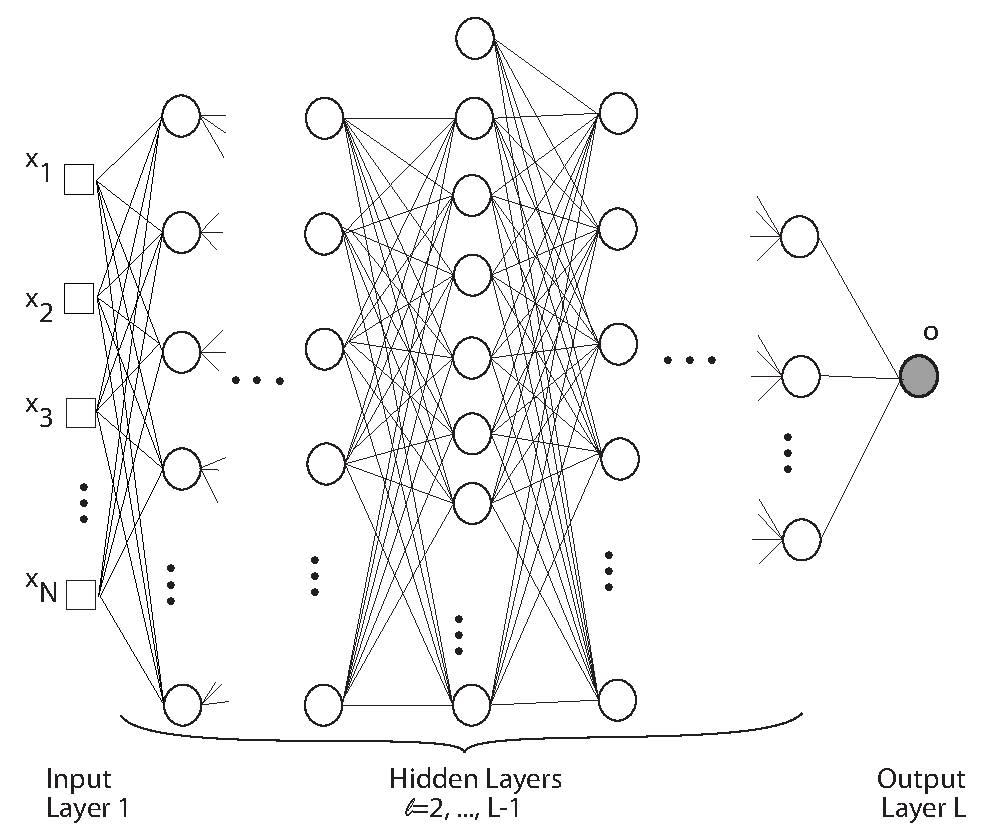
\includegraphics[scale=0.6]{mlp}
    \caption{Multilayer Perceptron with $L$ layers and a single node 
	     ($M\!=\!1$) on the output layer.}
    \label{f:mlp}
\end{figure}

Each training pattern $\vect{x}^{(t)}$ is presented to the sensory units of the input layer ($l\!=\!1$) and creates a signal that propagates towards the network output through the intermediate layers and, finally, reaches the last ($L$) layer node where the network response $o^{(t)}\!\doteq\!o(\vect{x}^{(t)})$ emerges. During the signal propagation, the input signal $h^{(t)}_{[q,l]}$ to the $q\!-\!th$ neuron in layer $l$ is processed by the nonlinear neuron model $\set{G}(h)$ and yields the neuron output $v^{(t)}_{[q,l]}$=$\set{G}(h^{(t)}_{[q,l]})$. A widely--used activation function is the logistic one, defined by
%
\begin{equation} \label{mlp_logistic}
   \set{G}(h)=\frac{1}{1+exp(-bh)}~,~~~-\infty\!<\!h\!<\!\infty~,~~~
   0\!<\!\set{G}(h)\!<\!1~,~~~B\!>\!1
\end{equation}
%
At any computational node (neuron $q$ lying in layer $l$; marked as $[q,l]$), the output signal $v^{(t)}_{[q,l]}$ is given by
%
\begin{equation} 
   v^{(t)}_{[q,l]}=
   \set{G} \left[ \sum_{s=1}^{K_{l-1}} w_{[q,l],[s,l-1]} v^{(t)}_{[s,l-1]} \right]
\end{equation}
%
expressing the output of the activation function on the weighted sum of all signals appearing at the outputs of the $K_{l-1}$ previous layer neuron outputs. 

The \MLP\ networks are trained in a supervised manner through the error back-propagation algorithm (\EBP) which is based on the error--correction learning rule. For the training, the $T$ paired samples $(\vect x^{(t)},\zeta^{(t)})$ are used. \EBP\ learning is an iterative algorithm which consists of forward (function) and backward (error) signal passing through the \MLP\ layers. In the forward pass, the input vector $\vect{x}^{(t)}$ of each training pattern is presented to the input layer and a signal propagates forward through the network. In the last layer, the network's prediction $o^{(t)}$ is compared to the known response $\zeta^{(t)}$ and the prediction error is computed. In the backward pass, the synaptic weights are corrected to minimize the prediction error.

%-----------------------------------------------------------------------
\subsubsection*{Kriging}
%-----------------------------------------------------------------------
\label{ss:krig}

Kriging belongs to the class of Gaussian random field metamodels. Kriging, \cite{Kri66}, may predict not only the response to a given input signal (such as a newly generated individual in an \EA) but, also, a measure of confidence (\emph{mean squared error}, \MSE) for this prediction, fig. \ref{f:krig}, \cite{Willmes2003}; 

As with the \MLP\ or \RBF\ networks, we assume that $T$ training patterns $\vect x^{(t)}\!\in\!\set{R}^N$, along with their responses $\vect{\zeta}^{(t)}\!\in\!\set{R}^M$ are available ant that $M\!=\!1$. In kriging, for any $\vect x\!\in\!\set{R}^N$, the corresponding response $o(\vect x)$ is expressed by
%
\begin{equation}
	o(\vect x) = \hat{\mu} + z \left( \vect{x} \right)
	\label{kr01}
\end{equation}
%
where $\hat{\mu}$ is the expected value and the covariance function $z \left( \vect{x} \right)$ is supposed to have zero mean and a user--defined correlation function $\set{C}$ with any other point in $\set{R}^N$.  So, the model output function becomes a realization of a random field $\set{F}$ that assigns a $1D$-Gaussian distributed random variable $\set{F}(\vect x)$ with constant mean $\hat{\mu}$ (the expected value of $\set{F}$) and variance $\sigma^2$ to each point in the search space. For two points $\vect{x}^{(\kappa)}$ and $\vect{x}^{(\lambda)}$, a typical choice for the correlation function is
%
\begin{equation}
  \set{C} \left(\vect{x}^{(\kappa)}, 
		\vect{x}^{(\lambda)},
		\vect{\theta}        \right) =
  \mbox{exp} \left( -\sum_{n=1}^{N} \theta_n
                     \left( x^{(\kappa)}_n - x^{(\lambda)}_n \right) ^2 \right)
\label{kr02}
\end{equation}
%
where the correlation parameters $\vect{\theta}=\left( {\theta_1},{\theta_2},...,{\theta_{_N}} \right) \in \set{R}^N$ must be computed in order to fit the model to the available data. Quite often, an isotropic correlation kernel is assumed and eq. \ref{kr02} is, then, rewritten with $\theta_n\equiv\theta$; in this case, a single $\theta$ value must be computed. Training the kriging model is the process of computing $\theta$'s, $\hat{\mu}$ and $\sigma^2$, which are all assumed to be invariant with respect to $\set{F}$.

According to the maximum likelihood hypothesis, the probability density function of $\set{F}(\vect x^{(t)})$ for each and every training pattern to be equal to its known response $\zeta^{(t)}$ must be maximized. This is mathematically expressed as
%
\begin{equation}
   \mbox{max} 
   \left[ \frac{1}{(2\pi)^{N/2} (\sigma^2)^{N/2} \sqrt{\det(\CBF)}} 
	  \exp \left[ \frac{(\vect{Z} - \onebf \hat{\mu})^T 
                            \CBF^{-1} (\vect{Z} - \onebf \hat{\mu})}
                           {2 \sigma^2} \right]
   \right]
   \label{kr03}
\end{equation}
%
where $\onebf$ is a column vector of length $N$ with unit entries and
%
\begin{equation}
   \CBF = 
   \left[
	\begin{array}{ccc}
	\set{C} \left(\vect{x}^{(1)}, \vect{x}^{(1)},\vect{\theta} \right)
	 &\cdots &
	\set{C} \left(\vect{x}^{(1)}, \vect{x}^{(T)},\vect{\theta} \right)\\
	\vdots& \ddots &\vdots\\
	\set{C} \left(\vect{x}^{(T)}, \vect{x}^{(1)},\vect{\theta} \right)
	&\cdots &
	\set{C} \left(\vect{x}^{(T)}, \vect{x}^{(T)},\vect{\theta} \right)
	\end{array}
   \right],\ 
   \onebf = 
   \left[
	\begin{array}{c}
	1\\
	\vdots\\
	1
	\end{array}
   \right],\
   \vect{Z} = 
   \left[
	\begin{array}{c}
	\zeta^{(1)}\\
	\vdots\\
	\zeta^{(T)}
	\end{array}
   \right]
   \label{kr04}
\end{equation}
%
The problem of eq. \ref{kr03} can be solved by adopting generalized least squares estimates for $\hat{\mu}$ and $\sigma^2$ , \cite{Koe96}, as follows
%
\begin{equation}
   \hat{\mu} = \frac {\onebf^T \CBF^{-1} \vect{Z}} 
		     {\onebf^T \CBF^{-1} \onebf}
   \label{kr05}
\end{equation}
%
\begin{equation}
   \sigma^2 = \frac {1}{N}(\vect{Z} - \onebf \hat{\mu})^T
   \CBF^{-1} (\vect{Z} - \onebf \hat{\mu})
   \label{kr06}
\end{equation}
%
The substitution of eqs.~\ref{kr05} and \ref{kr06} into eq.~\ref{kr03}, leads to the solution of an equivalent minimization problem,
%
\begin{equation}
    \mbox{min} \left[ (2\pi)^{N/2} (\sigma^2)^{N/2} 
		      \sqrt{\det(\CBF)} \exp(-\frac{N}{2}) \right]
    \nonumber
\end{equation}
%
or, finally,
%
\begin{equation}
   \mbox{min} \left[ N \ln \left( \sigma^2 (\vect{\theta}) \right) + 
                       \ln \left( \det \CBF(\vect{\theta}) \right)
              \right]
   \label{kr07}
\end{equation}
%
\begin{figure}
  \centering
  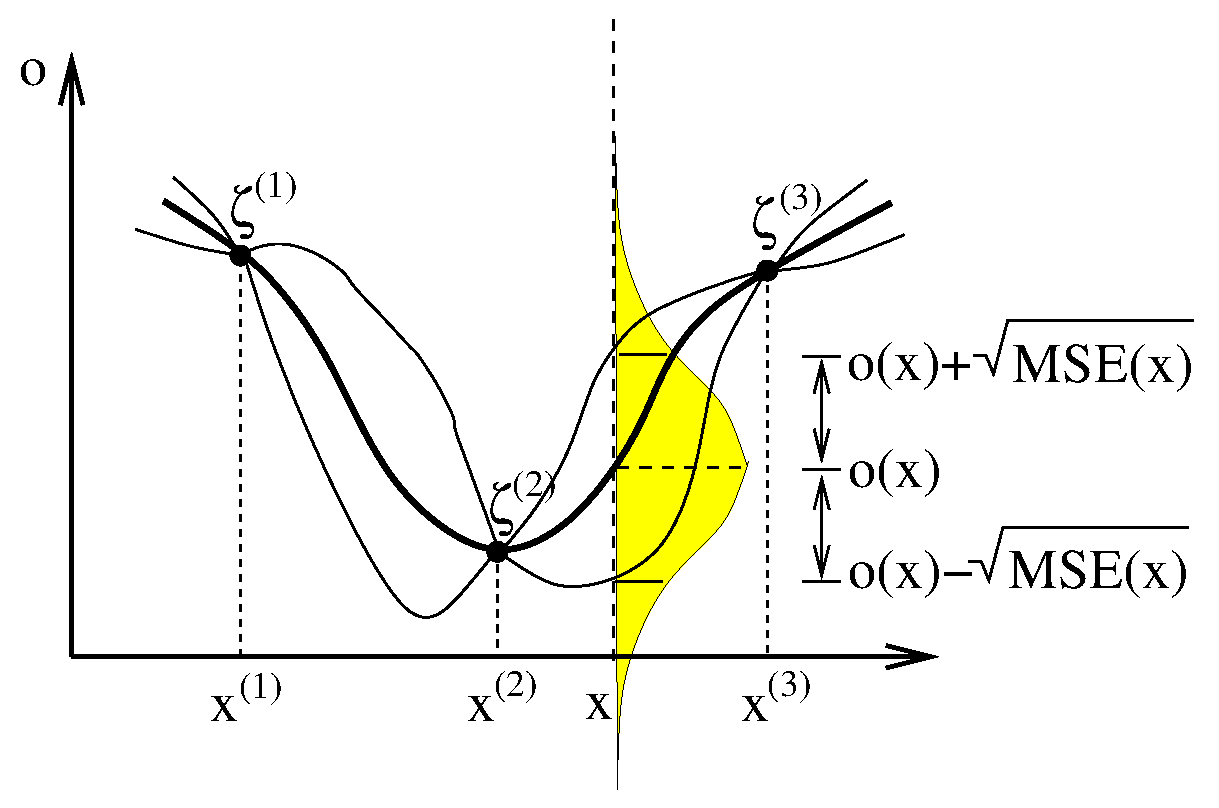
\includegraphics[scale=0.5]{krig}
  \caption{An $1$D example of the use of kriging. Based on three data points 
	   $(x^{(1)},\zeta^{(1)})$, $(x^{(2)},\zeta^{(2)})$ and 
	   $(x^{(3)},\zeta^{(3)})$, the response and the square root of the 
	   mean squared error for any other $x$ value can be computed.}
  \label{f:krig}
\end{figure}

After computing the $\theta$ values by solving the nonlinear problem of eq. \ref{kr07}, the corresponding response and \MSE\ predictions for any new $\vect x$ in the design space are, \cite{LTT_2_027},
%
\begin{equation}
   o(\vect{x})= \hat{\mu} + (\vect{Z} - \onebf \hat{\mu})^T \CBF^{-1} \cbf(\vect{x})
   \label{kr08}
\end{equation}
%
\begin{equation}
   \MSE(\vect{x}) = \sigma^2 \cdot (1-\cbf(\vect{x})^T\CBF^{-1}\cbf(\vect{x}))
   \label{kr09}
\end{equation}
%
see fig. \ref{f:krig}, where
%
\begin{equation}
   \cbf = \left[
   \set{C} \left(\vect{x}, \vect{x}^{(1)},\vect{\theta} \right),  \dots,
   \set{C} \left(\vect{x}, \vect{x}^{(T)},\vect{\theta} \right) \right]^T
   \label{kr10}
\end{equation}

%
%-----------------------------------------------------------------------
\subsubsection*{Polynomial--based regression surface methods (\RSM)}
%-----------------------------------------------------------------------
\label{ss:rsm}

A polynomial--based \RSM\ utilizes polynomials of user--defined order to model the function landscape. Unknown coefficients are introduced and their value set that best fits the training data is sought. This set is computed by solving a linear least--squares problem, i.e. a much easier process than the non--linear regression required for all the neural networks other than the \RBF\ ones. A polynomial--based \RSM\ can be used to filter noise out from experimental data and their only disadvantage is that they can hardly interpolate data corresponding to complex functions.

A first--order (linear) \RSM, with $N$ independent (design) variables or regressors is
%
\begin{equation}
   \vect{o(\vect{x})} = \beta_0 + \sum_{n=1}^N \beta_n x_n + \epsilon
\end{equation}
%
where $\beta_n,~n=0,\dots,N$ are the unknown regressor coefficients. 
Similarly, a second--order \RSM\ can be written as
%
\begin{equation}
   \vect{o(\vect{x})} = \beta_0 
			+ \sum_{n=1}^N \beta_n x_n
			+ \sum_{i=1}^N \beta_{ii} x_i^2 
			+ \sum_{i=1}^N \sum_{j=i+1}^N \beta_{ij} x_i x_j 
		        + \epsilon
\end{equation}
%
where, in both, $\epsilon$ is a random error.
Either of them can be written in matrix form as
\begin{equation}
   \vect{o(\vect{x})} = \vect{X} \vect{\beta} + \vect{\epsilon}
\end{equation}
%
The vector of least--squares estimators $\vect{\beta}$ that minimizes 
%
\begin{equation}
   \vect{\epsilon}^T \vect{\epsilon} =  (\vect{o} - \vect{X} \vect{\beta})^T
					(\vect{o} - \vect{X} \vect{\beta})  
\end{equation}
%
is sought; this leads to the least--squares normal equations and, though them, to
%
\begin{equation}
   \vect{\beta} =  (\vect{X}^T \vect{X})^{-1} \vect{X}^T \vect{o}
\end{equation}
%
The prediction performance of the trained \RSM\ can be quantified using various statistical measures. Further discussion on polynomial-based \RSM\ is beyond the scope of this lecture.
%
%#######################################################################
\section[MAEAs based on the IPE technique]
{MAEAs based on the IPE technique}
%#######################################################################
\label{s:MaeasIpe}

This section describes the implementation of on--line trained metamodels, according to the \IPE\ technique, on a generalized ($\mu,\lambda$) \EA, namely the EASY software, \cite{EASYsite}, which is the algorithm used for all the applications to be presented in this lecture.
In particular, the basic algorithmic steps of the ($\mu,\lambda$) \EA\ are presented, along with the ``changes'' due to the implementation of \IPE\ technique.
Due to its importance, the selection of the appropriate training patterns for the \RBF\ networks used as metamodels is discussed separately.

%=======================================================================
\subsection[The Evolutionary Algorithm SYstem]
{The Evolutionary Algorithm SYstem--EASY}
%=======================================================================
\label{ss:easy}

The set of design variables is designated by 
$\vect{x}\!\in\!\set{R}^N$ whereas
$\vect{F}(\vect{x})\!\in\!\set{R}^M$ denotes the objective function. 
In \MOO\ problems, for the approximation of the Pareto front of non--dominating solutions, a technique that maps $\vect{F}(\vect{x})$ into a scalar cost function value $\phi$ is additionally employed. For this purpose, \SPEA \cite{Zitz1999a}, \SPEAA \cite{Zitz2002}, \NSGA \cite{Sri1995}, \NSGAA \cite{Deb2000}, or any variant of them may be used. 
At each generation $g$, the ($\mu,\lambda$) \EA\ maintains and updates three populations, namely the offspring ($\set{P}_{\lambda,g}$) with $\lambda$ individuals, the parent ($\set{P}_{\mu,g}$) with $\mu$ individuals and the archival one ($\set{P}_\alpha$) of elite individuals. Furthermore, during the evolution, all previously evaluated (on the problem--specific model) individuals are recorded in a database (\DB).

%............................................................ 
\begin{namedalgorithm}{EASY}{Evolutionary Algorithm SYstem or $(\mu, \lambda)$ \EA}{}
%............................................................ 
%
%>>>>
\item[Initialization]\label{a:easyStart}
%>>>>
Set $g\!=\!0$ and randomly initialize the offspring population
$\set{P}_{\lambda,g}$.
%
%>>>>
\item[Offspring evaluation]\label{a:easyEval}
%>>>>
All ($\set{P}_{\lambda,g}$) members are evaluated on the 
problem--specific evaluation model and $(\vect{x},\vect{F}(\vect{x}))$ pairs 
are archived in the \DB. In constrained optimization problems, 
$\vect{F}(\vect{x})$ is penalized if any of the constraints is violated.
The penalty depends exponentially on the degree of the constraint violation.
%
%>>>>
\item[Cost ($\phi$) assignment]\label{a:easyFit}
%>>>>
For $\set{P}_g\!=\!\set{P}_{\lambda,g} \cup \set{P}_{\mu,g} \cup \set{P}_{a,g}$ members, $\phi(\vect{x})$ is computed through
%
\begin{equation}\label{e:costAssign}
     \phi(\vect{x}) = \phi(  \vect{F}(\vect{x}), %
                           \{\vect{F}(\vect{z})\ |\ %
                  \vect{z} \in\set{P}_g\setminus\{\vect{x}\}\}) %
                  \in \set{R}, \quad \vect{x} \in \set{P}_g
\end{equation}
%where $\hat{\vect{F}}(\vect{x})\!=\!\vect{F}(\vect{x})$.
Based on the $\phi(\vect{x})$ values the best offspring (current best for \SOO\ and non--dominated for \MOO) are singled out in the temporary set $\set{P}_e$.
Thinning algorithms can optionally be used to keep the $\set{P}_e$ population size less than a user--defined maximum value. 
The most frequently used criterion is the distance between them (measured in the objective space), in order to give priority to individuals at the less populated parts of the current front of non--dominated individuals.
%
%>>>>
\item[Elitism]\label{a:easyElit}
%>>>>
The elite population is updated through the elitism operator
$\op{E}$ applied to the union of $\set{P}_e$ and the previous elite archive
$\set{P}_{\alpha,g}$,
%
\begin{equation}
	\set{P}_{a,g+1} = \op{E}(\set{P}_{e} \cup \set{P}_{\alpha,g})
	\nonumber
\end{equation}
%
%>>>>
\item[Evolution]
%>>>>
New parents are selected using the selection operator $\op{S}$,
%
\begin{equation}
    \set{P}_{\mu,g+1} = \op{S}(\set{P}_{\mu,g} \cup
    \set{P}_{\lambda,g})
    \nonumber
\end{equation}
%
and new offspring are formed through the application of the crossover, $\op{C}$, and mutation, $\op{M}$, operators,
%
\begin{equation}
    \set{P}_{\lambda,g+1} = \op{M}(\op{C}(\set{P}_{\mu,g+1},
    \set{P}_{\alpha,g+1}))
    \nonumber
\end{equation}
%
%>>>>
\item[Termination] \label{a:easyTermin}
%>>>>
If the maximum number of exact evaluations is reached or the elite population does not change during the last generations, the algorithm terminates. 
Otherwise, $g\!\assign\!g\!+\!1$ and the algorithm continues from step \ref{a:easyEval}.
%...................
\end{namedalgorithm}
%...................

In distributed \EAs\ (\DEAs), the above algorithm is valid for each one of the semi--autonomously evolving sub--populations (the so--called \textit{demes} of \textit{islands}). 
The demes communicate according to a user-defined topology and exchange their best performing and, sometimes, a few randomly--selected individuals according to an inter--deme migration operator applied with a user--defined frequency. 

%=======================================================================
\subsection[Use of the Inexact Pre--Evaluation within the $(\mu, \lambda)$ EA]
{Use of the Inexact Pre--Evaluation within the $(\mu, \lambda)$ EA}
%=======================================================================
\label{ss:ipe}

\IPE\ is a low--cost screening technique applied within each generation, 
\cite{LTT_3_054, LTT_2_029}.
In specific, the entire population is pre--evaluated on locally trained metamodels and only a few top individuals among them are, then, re--evaluated on the problem--specific model (see fig. \ref{f:on-line-ipe}).

\begin{figure}
    \centering
    \includegraphics[scale=0.7]{on-line_ipe}
    \caption{The \IPE\ algorithm based on on--line trained local metamodels 
	     used to filter the offspring population at each generation, so 
	     that only a small fraction of it to be re--evaluated on the 
	     costly problem--specific model.}
    \label{f:on-line-ipe}
\end{figure}
%
The algorithm starts as a conventional $(\mu, \lambda)$ \EA\ (by, exclusively, making use of the exact evaluation model) for the few starting generations until a user--defined minimum number of exact evaluations enter the \DB. 
Then, the \IPE\ phase starts and, in subsequent generations, instead of evaluating the offspring population on the costly, problem--specific model (as in step \ref{a:easyEval}), the following actions are taken:
%
%....................................................
\begin{namedalgorithm}{IPE}{Inexact Pre-Evaluation}{}
%....................................................
%>>>>
\item[Inexact evaluation]
%>>>>
For each offspring, $\vect{x}\!\in\!\set{P}_{\lambda,g}$, the objective function values $\apprx{\vect{F}}(\vect{x})$, are approximated using a local metamodel trained on a small number of data selected from the \DB. 
The selection of the training set is described in section \ref{tps}. 
%
%>>>>
\item[Screening]\label{a:ipeSelect}
%>>>>
Based on the $\apprx{\vect{F}}(\vect{x})$ values, a provisional
$\phi$ value (denoted by $\apprx{\phi}$) is assigned to each
offspring
%
\begin{equation} \label{e:cost-tmp}
   \apprx{\phi}(\vect{x}) = \apprx{\phi}(\apprx{\vect{F}}(\vect{x}), %
   \{\apprx{\vect{F}}(\vect{z})\ |\ %
   \vect{z} \in\set{P}_{\lambda,g}\setminus\{\vect{x}\}\}) %
   \in \set{R}, \quad \vect{x} \in \set{P}_{\lambda,g}.
\end{equation}
%
In \SOO\ problems, $\apprx{\phi}(\vect{x})\!\equiv\!\apprx{\vect{F}}(\vect{x})$.
In \MOO\ problems, the assignment method of step \ref{a:easyFit} can be used, i.e. by using $\vect{F}(\vect{x})$ instead of $\apprx{\vect{F}}(\vect{x})$.
However, since $\apprx{\vect{F}}(\vect{x})$ is just an approximation to 
$\vect{F}(\vect{x})$ and due to the large number of comparisons required by 
any scalar cost assignment technique (\SPEA, \NSGA, etc),
it is recommended to compute $\apprx{\phi}$ using the simplest possible scheme.
Irrespective of the scheme used in step \ref{a:easyFit}, a simple ranking in
non--dominated fronts (without sharing) often suffices. Based on the
so--computed $\apprx{\phi}$ values, the best $\lambda_e\!<\!\lambda$
($\lambda_e\!=\!s \lambda$, where $s\!\ll\!1$ is user--defined) offspring are singled out in the 
temporary set $\set{P}_{e}$,
%
\begin{equation}
    \set{P}_{e} \defeq \{ \vect{x}_i, \medspace i=1,2,\dots,\lambda_e :
    \apprx{\phi}(\vect{x}_i) < \apprx{\phi}(\vect{z}), 
    \medspace \vect{z} \in \set{P}_{\lambda,g}\setminus\set{P}_{e}\}.
    \nonumber
\end{equation}
%
%>>>>
\item[Exact evaluation]
%>>>>
For all $\vect{x}\!\in\!\set{P}_{e}$, the exact objective function values $\vect{F}(\vect{x})$ are computed and stored in the \DB. 
Practically, this step, determines the \CPU\ cost of each generation.
%
%...................
\end{namedalgorithm}
%...................
%
\noindent
During \IPE, in step \ref{a:easyFit}, eq. \ref{e:costAssign} is applied by using either the exact ($\vect{F}(\vect{x})$) or the approximate ($\apprx{\vect{F}}(\vect{x})$) objective function values, depending on whether each individual has been evaluated on the exact model or only the metamodel.

In the \IPE\ phase, various metamodels, either global (periodically retrained or updated, \cite{Jin2004}) or local (constructed on the fly for each and every individual, using the most appropriate subset of the available data, \cite{LTT_2_023}) can be used. 
However, practice has shown \cite{LTT_3_054, LTT_2_018} that local metamodels generally provide better predictions, especially in cases with complex objective function landscapes. 

The implementation of the \IPE\ phase within a \DEA\ is straightforward, since the same evaluation model is used within all sub--populations and a \textit{common} \DB\ of previously evaluated individuals is maintained. 
This means that the patterns used for training a local metamodel for any individual belonging to any deme may have been evaluated by any other deme.
%
%
%=======================================================================
\subsection[Selection of Training Patterns]
{Selection of training patterns for local metamodels}
%=======================================================================
\label{tps}

An important issue that affects the prediction ability of local metamodels is the selection of the most appropriate training patterns, from the \DB\ of previously evaluated individuals. 
For each individual $\vect{x}\!\in\!\set{R}^N$ to be pre--evaluated on the metamodel, the corresponding training pattern set $\set{T}$ must ``optimally'' be populated. 
The number $T$ of training patterns may vary between user--defined lower ($T_{min}$) and upper ($T_{max}$) bounds. 

An easy way to populate $\set{T}$ is by selecting $T$ \DB\ entries lying in the vicinity of $\vect{x}$, based on distances measured in the non--dimensional design space. 
In \MOO\ problems, populating $\set{T}$ is much more demanding.
When seeking the Pareto front, the local metamodels should provide accurate predictions along a front of solutions and not only around a single point which is likely close to the sought optimal solution.
Furthermore, in \MOO\ problems, the identification and special treatment of \emph{outliers}, i.e. new individuals that are far apart from most of the \DB\ entries, fig. \ref{tps:tps_example}, is very important.
For the outliers, since it is difficult to form an adequate training set, the problem--specific model must be used. 
An algorithm to identify outliers is required.
%
\begin{figure}[h!]
    \centering
    \includegraphics[scale=1.0]{tpsExample.eps}
    \caption{Example of a new individual (filled square) for the
	pre--evaluation of which a dependable training set (with four
	training patterns located within a circle of user--defined radius)
	can be found. This figure also shows an outlier (empty square) that
	must be identified and, then, evaluated on the
 	problem--specific model. It is assumed that $\vect{x}\!\in\!\set{R}^2$
	and that the two design variables $x_1$ and $x_2$ are 
	nondimensionalized.}
    \label{tps:tps_example}
\end{figure}
%

Below, a well performing (in either \SOO\ or \MOO) algorithm, is presented, \cite{LTT_2_029}. 
For each new individual $\vect{x}$, for which a metamodel is to be built, its closest neighbors in the design space are retrieved from the \DB\ to form a temporary pool ($\set{T}_{pool}$).
For the gathered points, including $\vect{x}$, the corresponding minimum length spanning tree (\MST, \cite{Knu97}) is generated. The \MST\ connects all these points with a line of minimum total length. 
Then, each \MST\ branch is traversed and, depending on a number of criteria, a point may be cut off.
Points which finally remain on the tree form the training set. 
The basic steps of this algorithm are described below:

%.........................................................
\begin{namedalgorithm}{TPS}{Training pattern selection}{}
%.........................................................
\item[Pool formation]\label{a:tps-poolform}
    An initial pool $\set{T}_{pool}$ of \DB\ members which are close to $\vect{x}$ is formed. As rule of the thumb, the size of $\set{T}_{pool}$ must be $3$ to $4$ times larger than $T$.
%
\item[Pool Thinning]\label{a:tps-poolthin}
    The \MST\ for the $\set{T}_{pool}$ members is created. \MST\ branches with length below a user--defined value are consolidated by eliminating the ending point with the minimum distance to any other individual within the pool.
When a branch is eliminated, the \MST\ is updated and the process is repeated until all branches satisfy the minimum length criterion.
%
\item[Treatment of outliers]\label{a:tps-poolout}
    From the data points left on the \MST, the $T_{min}$ patterns which are closer to the new individual are selected. If the closest pattern to $\vect{x}$ is at distance greater than a user--defined trust region radius, $\vect{x}$ is marked as \emph{outlier}. 
This radius is either equal to the \MST\ average branch length plus a tolerance expressed in terms of the corresponding standard deviation or proportional to the design space size.
%
\item[Complementary data]\label{a:tps-finalts}
    Depending on the structure of the closest data points, more data points may enter $\set{T}$, without however exceeding the upper bound of $T_{max}$ patterns.
%...................
\end{namedalgorithm}
%...................
%
%
\begin{figure}[h!]
    \centering
    \begin{minipage}{0.49\linewidth}
        \includegraphics[scale=1.0]{stp_goodrbf_st1.eps}
        \vspace{0.3cm}
    \end{minipage}
    \begin{minipage}{0.49\linewidth}
        \includegraphics[scale=1.0]{stp_goodrbf_st2.eps}
        \vspace{0.3cm}
    \end{minipage}
%
    \begin{minipage}{0.49\linewidth}
        \includegraphics[scale=1.0]{stp_badrbf_st2.eps}
    \end{minipage}
    \begin{minipage}{0.49\linewidth}
        \includegraphics[scale=1.0]{stp_outrbf_st2.eps}
    \end{minipage}
    \caption{Indicative cases of training pattern selection in a
            problem with two design variables $(x_1,x_2)$, according
            to the \emph{TPS} algorithm. It is assumed that 
	    $\vect{x}\!\in\!\set{R}^2$.}
    \label{tps:tps_mst}
\end{figure}

Fig. \ref{tps:tps_mst} presents snapshots of the use of the
\emph{TPS} algorithm in a problem with two design variables. The new
individual $\vect{x}$ is denoted by a black square and the \DB\
entries with empty circles. Points marked with a cross designate the
closest neighborhood to the individual, whereas the final training
set $\set{T}$ is shown with filled circles. The \MST\ drawn is
designated by solid lines. The first case (fig. \ref{tps:tps_mst},
top) is expected to give a dependable training set. After creating
the \MST\ (top--left), the thinning process leads to a reduced \MST\
(top--right). A circle of user--defined radius serves to finally
select the training patterns (top--right). Fig. \ref{tps:tps_mst}
(bottom--left) shows an individual failing to form a dependable
training set, since most of the available data points fall outside
the circle. Thus, any metamodel trained on these few patterns is
expected to provide quite inaccurate guesses. An outlying individual
is shown at fig. \ref{tps:tps_mst} (bottom--right). 

%
%=======================================================================
\subsection[Application of MAEAs]
{Application of MAEAs}
%=======================================================================
\label{s:maeasapp}


Below, four aero/hydrodynamic optimization problems, either \SOO\ or \MOO, are presented.
Through these problems, it is convincingly shown that the use of surrogate evaluation models to support an \EA, based on the \IPE\ technique (i.e. a \MAEA) constantly outperforms conventional \EAs. In addition, the last two cases demonstrate that one can further improve the performance of \EAs\ and \MAEAs\ using the \textit{principal component analysis} technique.

%
% 4-element SOO
%
\xeraki The first case is dealing with the optimal deployment of a four--element airfoil for maximum lift coefficient ($C_L$) at $M_{\infty} = 0.2$, $a_{\infty}=10^o$ and an inviscid fluid. The design variables stand for the relative positions of the slat and the two flaps with respect to the main body of the airfoil (fig. \ref{f:elemDesc}). In particular, for each but the main element, the design variables are its two displacements (horizontal and vertical) along with a rotation angle, summing up to $3\!\times\!3\!=\!9$ design variables, in total.
The evaluation software is the \GPU\ implementation of an in--house Euler equations solver \cite{LTT_2_047, LTT_2_051}, for compressible flows that employs a time--marching, vertex--centered, finite volume scheme on unstructured grids. 
For this problem, the mixed precision arithmetic variant \GPUM\ which uses single precision arithmetic for the l.h.s. coefficient matrices and double precision arithmetic for the residuals, was used; compared to its \CPU\ counterpart this code is faster by about $90\times$.
The optimization was carried out using both a ($20, 50$) \EA\ and a ($20, 50$) \MAEA\ in which $\lambda_e\!=\!6$ out of the $\lambda\!=\!50$ pre--evaluated offspring were re--evaluated on the Euler solver. The stopping criterion was set at $1000$ evaluations on the \GPUM\ code. An NVIDIA \GPU\ cluster was used.
In the \MAEA, the \IPE\ phase began after the first $100$ candidate solutions were stored in the \DB.
Comparison of the convergence histories of \EA\ and \MAEA\ runs is presented in fig. \ref{f:elemConv}. From this figure, it is concluded that the \MAEA\ is about three times faster than the \EA. The Mach field on the optimal solution computed with \MAEA\ is shown in fig. \ref{f:elemRes}.

\begin{figure}[ht!]
    \centering
    \includegraphics[scale=1.3]{maeas/4elemDesc.eps}
    \caption{Optimal deployment of a four--element airfoil for maximum lift 
	coefficient. Definition of the design variables (displacements and 
	rotation) that define the relative positions of the slat and the two 
	flaps with respect to the main body.}
    \label{f:elemDesc}
\end{figure}
%
\begin{figure}[ht!]
    \centering
    \includegraphics[scale=1.5]{maeas/4elemEaMaea.eps}
    \caption{Optimal deployment of a four--element airfoil for maximum lift 
	     coefficient. The convergence history of the \SOO\ problem is 
	     plotted in terms of the number of exact evaluations, i.e. 
	     the number of Euler computations which is proportional to the
	     \CPU\ cost.}
    \label{f:elemConv}
\end{figure}
%
\begin{figure}[ht!]
    \centering
    \includegraphics[angle=-90,scale=0.5]{maeas/4elemRes.eps}
    \caption{Optimal deployment of a four--element airfoil for maximum lift 
	coefficient. Mach field for the optimal solution computed with 
	\MAEA.}
    \label{f:elemRes}
\end{figure}
%

%
%   MAN MOO
%
\xeraki The second case is concerned with the shape optimization of a compressor cascade for minimal total pressure losses, while maintaining an acceptable performance level at off-design flow conditions.
The two objectives are 
%
\begin{align}
    &\mbox{min}~F_1 =  \omega_{\alpha_1}^{(OP_1)} =
            \frac{p_{t1}-p_{t2}}{\frac{1}{2} \rho_1 V_1^2}
    \nonumber \\
    &\mbox{min}~F_2 = 10^4 \cdot \{
    ( \omega_{\alpha_1}^{(OP_2)}-\omega_{\alpha_1}^{(OP_1)} )^2 +
    ( \omega_{\alpha_1}^{(OP_3)}-\omega_{\alpha_1}^{(OP_1)} )^2
    \}
    \nonumber
\end{align}
%
where $OP_1$ denotes the design operating point with 
$\alpha_1^{(OP_1)}\!=\!47^o$ and $OP_2$, $OP_3$ are two off--design
points with $\alpha_1^{(OP_2)}\!=\!43^o$ and $\alpha_1^{(OP_3)}\!=\!51^o$
respectively. In all operating points $M_1\!=\!0.62$ and $Re\!=\!8.41\cdot10^5$. 
The evaluation model used for this case is an integral boundary layer software ($CFD-IBL$)\footnote{Drela's MISES analysis software, \cite{Drel1987}, based on an integral boundary layer method coupled with an external inviscid flow solver.}. 
The design variables are the coordinates of the NURBS control points parameterizing the airfoil. 
Geometrical constraints on the minimum airfoil thickness, the radius of curvature at the leading edge and the angles between the first pressure/suction side control points and the leading edge were imposed. 
The flow exit angle must be kept between $19^o$ and $21^o$ and this was imposed as constraint. 

%
\begin{figure}[!ht]
    \centering
    \includegraphics[scale=1.5]{maeas/manConv.eps}
    \caption{Shape optimization of a compressor cascade airfoil. Convergence
             history of the \textit{hypervolume indicator} $I_H$ (a metric of 
             the quality of the computed front; greater metric value 
	     denotes a ``better'' front of non--dominating solutions).
             This case demonstrates that, in \MOO\ problem, the use of 
             \SOMs\ for the selection of \RBF\ centers during training
             (as discussed in section \ref{ss:RBF}) performs better than 
             the conventional \RBF\ networks trained on just the immediate 
	     neighbors. From \cite{LTT_3_075}.}
    \label{f:manConv}
\end{figure}

In this case, some difficulties arose due to the imposition of severe constraints and the inability of the evaluation tool to cope with massively separated flows, which are likely to occur at off--design conditions (at least for several intermediate airfoil shapes evaluated during the evolution). 
These difficulties resulted in a high number of failing evaluations; indeed, approximately $350$ out of the $2000$ evaluations failed. 
Nevertheless, the \IPE\ phase proved to be quite robust and reduced the computational effort required for generating a front of given quality, fig. \ref{f:manConv}. 
In fig.  \ref{f:manFront}, the front obtained from the \MAEA\ is compared with that achieved by a conventional \EA; also, three representative solutions belonging to the front are shown.

\begin{figure}[!ht]
    \centering
    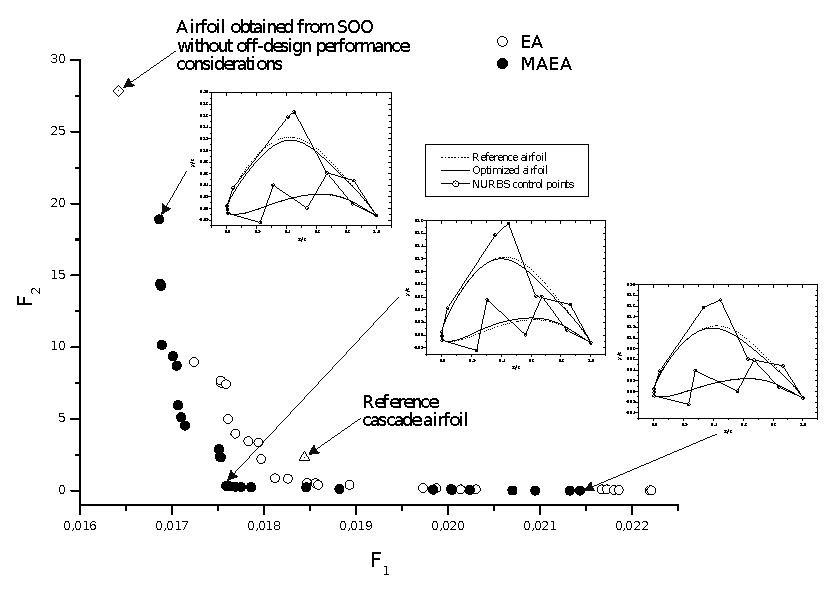
\includegraphics[]{maeas/manFront.eps}
    \caption{Shape optimization of a compressor cascade airfoil. Non--dominated
            fronts after $2000$ exact evaluations using \EA\ and \MAEA\
            (\EA\ with \IPE), along with a couple of selected optimal cascade 
   	    airfoils obtained by the \MAEA. From \cite{LTT_3_075}. The front 
	    computed using the \MAEA\ practically dominates all the front 
	    members computed by the conventional \EA\ at the same \CPU\ cost.}
            \label{f:manFront}
\end{figure}

%
% MAN Stelios PCA
%

\xeraki The third case is concerned with the shape optimization of a (different) compressor cascade airfoil for minimum total pressure losses $\omega$. 
The cascade operates at the following flow conditions: $M_1\!=\!0.54$, 
$a_1\!=\!44^o$, $Re\!=\!4\cdot10^5$ and has an axial--velocity--density--ratio equal to $1.12173$. The stagger angle is fixed and equal to $20^o$.
The airfoil mean curvature line was parameterized using three design variables and the thickness distribution was then parameterized using $9$ design varables for the pressure and $15$ for the suction side. 
The total number of design variables sums up to $27$.
Geometrical constraints on the airfoil thickness at three chord--wise positions ($t^{0.4c}\geq0.1$, $t^{0.6c}\geq0.08$ and $t^{0.9c}\geq0.01$) and an additional constraint on the flow turning (to be greater than $30^o$) were
imposed. The evaluation tool is the same $CFD-IBL$ software.

This \SOO\ case was studied not only for demonstrating, once more, that a \MAEA\ outperforms the standard \EA\ but, also, for proceeding beyond the \MAEAs\ described thus far. In this respect, a new enhanced variant of \MAEAs, which additionaly employs the \textit{principal components analysis} (\PCA) of the design variables' vector, was devised and used in this problem. Thus far, \PCA\ has found application in pattern recognition or image compression techniques, for handling data sets of high dimension \cite{Hayk1999}. \PCA\ is the process of transforming a data set in such a way that the transformed data set can be represented by a reduced number of ``effective'' features, without damaging the ``useful'' contents of the original data set. Practically, \PCA\ is nothing but a ``smart'' coordinate transformation of points in the data space to points in the so--called feature space. The rotated vector corresponding to a point in the feature space can optionally be truncated; it can be proved that the rotation ensures maximum rate of decrease in variance; so, this truncation is capable of maintaining the maximum of the information contained into the original data set.

One way of using the \PCA\ during an EA-- or \MAEA--based optimization is for improving the performance of the evolution operators. An \EA\--based method performs better if applied onto functions with \textit{separable} design variables. By definition, a function of separable variables can be written in components, each of which depends on a single design variable; thus, in a problem with $N$ optimization variables, the minimization of the objective function is equivalent to the minimization of $N$ $1\!-\!D$ functions. Therefore, the minimization of functions with separable variables is not subject to the curse of dimensionality. Using \PCA, the design variable space is rotated, so as to make the design variables of the objective function under consideration as separable as possible. In different words, this could be understood as the process of rotating the axes of the design space so as to come up with a new set of the ``most important'' directions; no truncation takes place. This can be done for all the population members just before employing the evolution operators. After the application of the evolution operators, the opposite rotation is necessary so as to return the new offspring population members in the standard coordinate system (according to the selected parameterization). The new variant will be denoted by \EA(\PCA) or \MAEA(\PCA), depending on whether metamodels are also used.

Based on the above, this problem was solved twice, using \MAEA\ and \MAEA(\PCA). The reason is to demonstrate that the \MAEA's performance can further be improved using the \PCA\ technique. The comparison is shown in fig. \ref{f:PCAcasc}. \MAEA(\PCA) is much faster than MAEA.

\begin{figure}[!ht]
    \centering
    \includegraphics[scale=1.4]{maeas/CascPCA.eps}
    \caption{Shape optimization of a compressor cascade airfoil for minimum 
	     total pressure losses at the nominal operating point. 
	     Comparison of the convergence history of \MAEA\ with and without 
	     \PCA.}
    \label{f:PCAcasc}
\end{figure}

%
%  Matrix Steliou
%
\xeraki The last case is dealing with the design--optimization of a Hydromatrix\textregistered\footnote{Hydromatrix\textregistered~is a new innovative concept of low--head hydraulic energy generation developed by Andritz HYDRO. It can be easily integrated into existing dam structures or weirs, combining the advantages of low cost installation and minimal environmental impact since no new civil structures are needed. The Hydromatrix\textregistered~system utilizes a factory assembled ``matrix'' or module of small (with diameter ranging from $0.9$ to $1.3$ meter), axial flow, fixed blade (``unregulated'') turbine generator units instead of a larger conventional ``regulated'' one.  The discharge regulation  of a Hydromatrix\textregistered~power plant is achieved by taking single units in or out of operation depending on the need to either increase or decrease the per unit discharge. www.andritz.com} turbine runner at three operating points (part load, full load and best efficiency point).
The design was performed by designers/engineers of Andritz HYDRO at Linz, Austria using the optimization software EASY.
The runner has $4$ blades and each runner blade is parameterized via superimposing a thickness distribution onto a mean camber surface, fig. \ref{f:MatParam}. 
The blade thickness distribution is chosen based on the expected structural stresses exerted to the blade and is fixed during the optimization. Therefore, the runner blade shape is controlled by the parameters defining its mean camber surface. 
The design variables are the coordinates of the control points of the Bezier curves used to parameterize the spanwise distributions of (a) the mean camber surface angles at the leading (LE) and trailing (TE) edges, (b) the circumferential position of the blade LE and TE and (c) the mean camber surface curvature. Overall, there are $52$ design variables and the same \MAEA\ assisted by \PCA\ was used.

\begin{figure}[!ht]
    \centering
    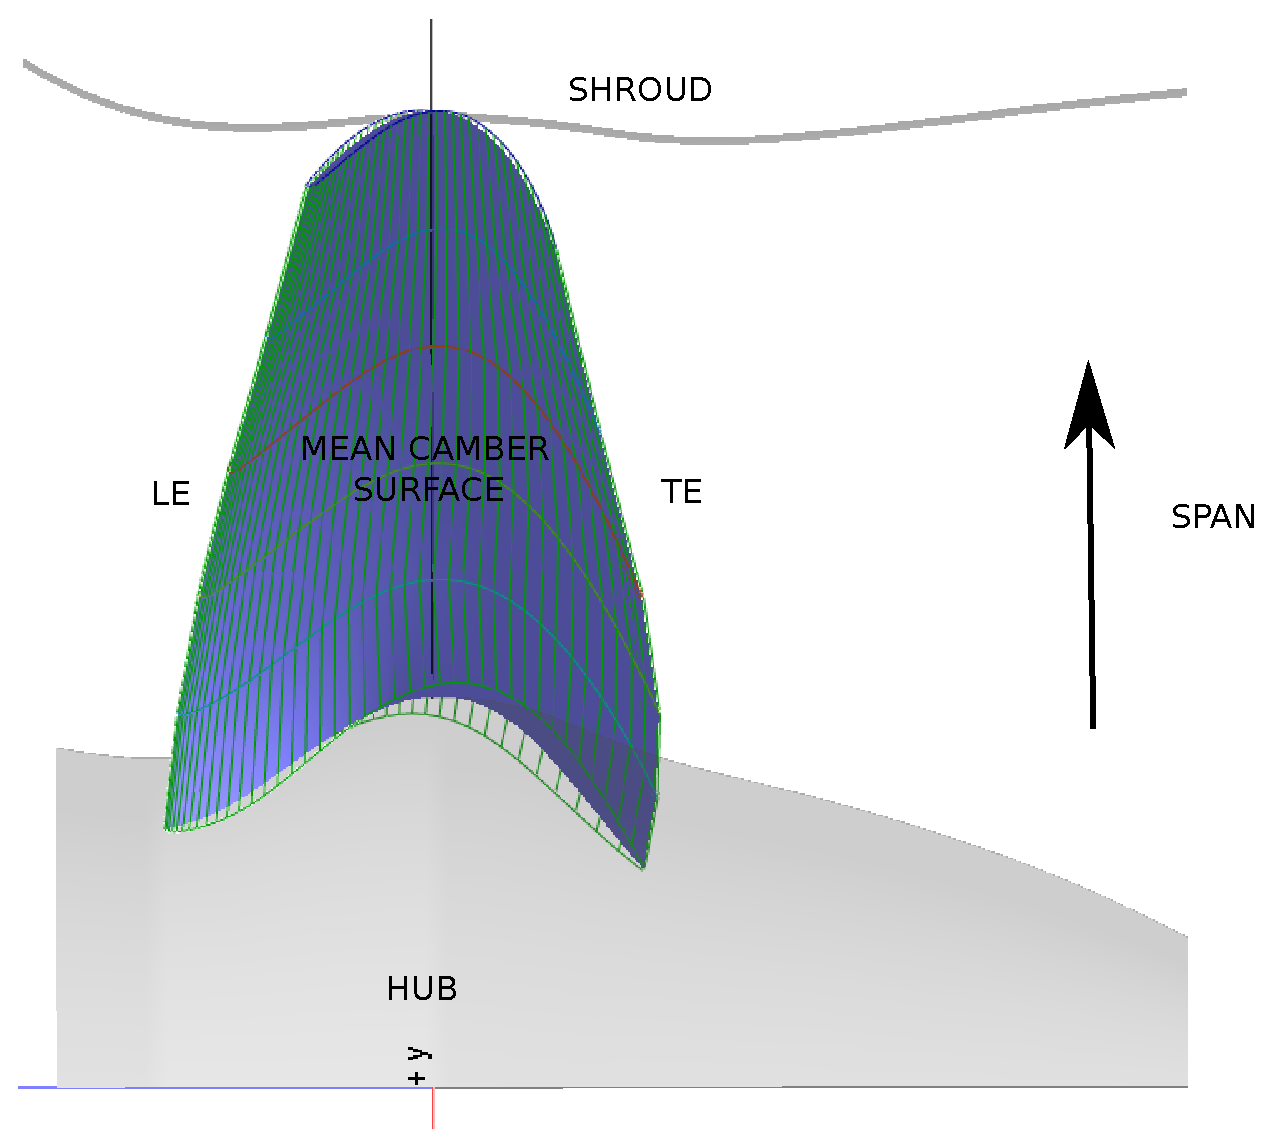
\includegraphics[angle=0, scale=0.4]{maeas/MatrixParam.eps}
    \caption{Parameterization of a Hydromatrix\textregistered~runner blade.
             Eleven blade profiles in the spanwise direction generated on
	     the mean camber surface using known thickness distributions 
	     and the surface grid of the blade are shown.}
    \label{f:MatParam}
\end{figure}

For each operating point, three metrics are used to measure the runner flow quality. The first metric ($f_1$) quantifies how close the velocity profile at the runner outlet is to the recommended one at the existing draft tube inlet. Given that the draft tube is fixed, known swirl and axial velocity profiles at the exit of the runner are required; from this point of view, metric $f_1$ becomes the objective function of an inverse design problem in which the target velocity components' distribution is defined at the runner exit. The second metric ($f_2$) is related to the blade loading which must be uniform (i.e. with minimum variations) over the blade surface. The third metric ($f_3$) quantifies the cavitation danger for the blade based on a safety margin defined by the designer. 
This case was studied as a two--objective constrained optimization problem. The weighted sum (for all the three operating points) of metrics $f_1$, $f_2$ were used as objective functions
\begin{equation}
	F_1 = \sum_{i=1}^3 w^{OP_i} f_1^{OP_i} ~~\mbox{,}~~ 
	F_2 = \sum_{i=1}^3 w^{OP_i} f_2^{OP_i}
        \nonumber
\end{equation}
with $w^{OP_1}=1.0,~ w^{OP_2}=0.1,~ w^{OP_3}=0.1$, while $f_3$ was imposed as a constraint.

Optimization runs were carried out using a ($30, 90$) \MAEA\ with $\lambda_e\!=\!18$. 
The \IPE\ phase was activated after the first $300$ non--failed evaluations were stored in the \DB. In the case of \MAEA\ assisted by \PCA, the \PCA--assisted evolution operators were applied after the $5^{\mbox{th}}$ generation. 
The resulting fronts of non--dominated solutions are compared in fig. \ref{f:MatRes} (left) where it is obvious that the use of \PCA\ is very important in such a high--dimensional problem. A selected geometry (point $A$) from the front resulted from the \MAEA(\PCA) is shown in fig. \ref{f:MatRes} (right). For point $A$, the whole Hydromatrix\textregistered~geometry is shown, including both the runner that was optimized (with its $4$ blades) and the stator which was known beforehand.

%
\begin{figure}[!ht]
    \begin{minipage}{0.49\linewidth}
        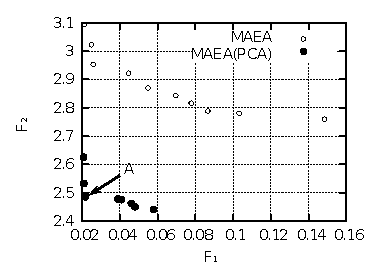
\includegraphics[scale=1.3]{maeas/MatrixPareto.eps}
        \vspace{0.3cm}
    \end{minipage}
    \begin{minipage}{0.49\linewidth}
        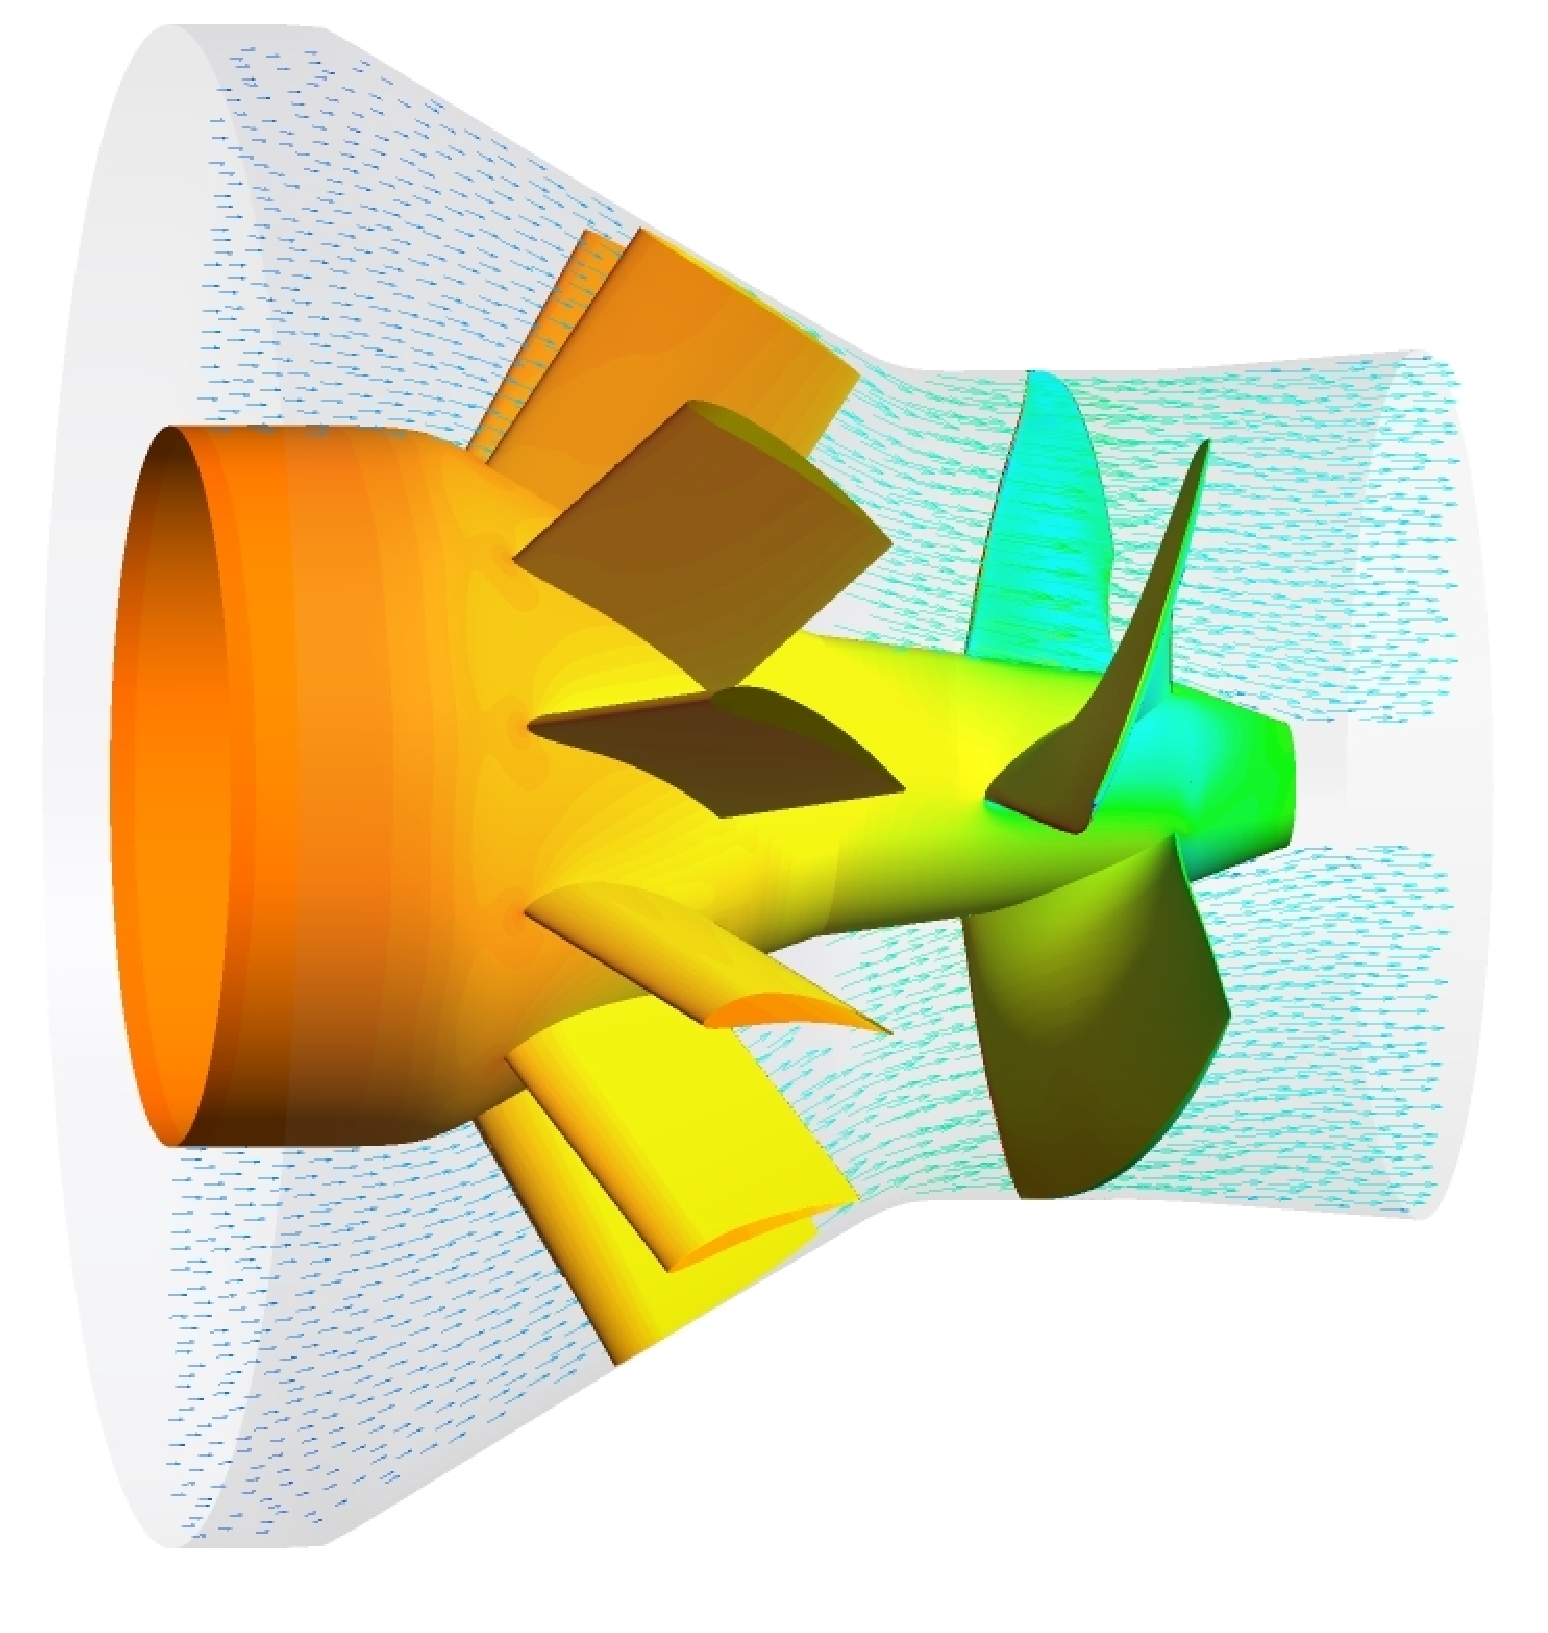
\includegraphics[scale=0.3]{maeas/MatrixFlow.eps}
        \vspace{0.3cm}
    \end{minipage}
    \caption{Two--objective optimization of a Hydromatrix\textregistered~ 
	     runner. Comparison of the front of non--dominated solutions 
	     obtained with \MAEA\ and \MAEA(\PCA) (left). The pressure field
	     is plotted over the geometry corresponding to point $A$ (right). 
             For $A$, the runner and the stator (which remained constant 
	     during the optimization) are shown. From \cite{LTT_2_054}.}
    \label{f:MatRes}
\end{figure}

%
%
%#######################################################################
\section[Hierarchical EAs and MAEAs]
{Hierarchical EAs and MAEAs}
%#######################################################################
\label{s:HMAEA}

As mentioned in the introduction, another way to reduce the wall clock time of an optimization problem is by means of hierarchical schemes. 
This section presents various concepts of hierarchical structures and applications of \HEAs\ and \HMAEAs.

%=======================================================================
\subsection{HEAs: Basic Concepts}
%=======================================================================
\label{ss:HEA}

The hierarchical structure requires the definition of a number of semi--autonomously ``evolving'' levels. In this multilevel structure, each level can be associated with different evaluation tools, search techniques and/or problem parameterizations, 
\cite{Herr1999, Sefr2000, Desid2003, LTT_2_031, LTT_3_092, LTT_2_036,
LTT_2_044, LTT_2_048, LTT_4_05}. 
Adjacent levels exchange their best individuals using one-- or two--way 
inter--level communications.
Depending on the type and timing of inter--level communications, the terms ``hierarhical'' or ``multilevel'' optimization might or might not mean the same. The most frequenlty used algorithms are those based on two levels only.

\subsubsection*{Hierarchical Evaluation Scheme}

In the \textit{hierarchical evaluation scheme} a different evaluation tool/software is assigned to each level. By convention, the lower level undertakes the exploration of the design space, i.e. the detection of near--optimal solutions at low \CPU\ cost before delivering them to its higher level for further refinement and so forth. 
Thus, inexpensive, low--fidelity evaluation models are usually associated with the lower levels. On the higher level(s), which are exploitation oriented and the uppermost of them is responsible for delivering the optimal solution(s), evaluation models of higher fidelity and \CPU\ cost are employed. 
A two--way inter--level communication can optionally be used allowing (apart from the migration of promising individuals upwards for them to undergo refinement) other individuals to move downwards to stimulate a more exhaustive search in their neighborhood, based on lower cost evaluation tools.

\subsubsection*{Hierarchical Search Scheme}

In the \textit{hierarchical search scheme}, each level is associated with a different search technique. Any combination of stochastic/heuristic and gradient--based methods can be used. Stochastic search techniques, such as \EAs\ (\DEAs, \DMAEAs, etc.), are preferably used on the low level for the exploration of the design space.  Promising solutions migrate to the high level, which is usually (but not necessarily) associated with a gradient--based method for their refinement.  The migration of promising solutions is, preferably, bi--directional so as to accentuate the exploration capabilities of low--level \EAs.

\subsubsection*{Hierarchical Parameterization Scheme}

The \textit{hierarchical parameterization scheme} associates coarse and fine problem definitions with each level. The coarser definition (reduced number of design variables and/or relaxed constraints) corresponds to the low level, where rough designs are quickly detected due to the small dimensionality of the problem. The hierarchical or multilevel parameterization scheme must be configured in a way that makes all but the highest level not affected (or, at least, slightly affected) by the curse of dimensionality. During the inter--level migration steps, a few promising solutions detected on the low level(s) are forwarded to the higher level(s) for refinement. This hierarchical scheme is suitable for shape optimization problems in which the design vector is formed by the coordinates of the control points of the parametric curves and surfaces since, by increasing or decreasing the number of control points via knot insertion and removal algorithms \cite{NURBSBook} allows exact (upwards) or approximate (downwards) transformations of the design vectors.

\begin{figure}[h!]
    \centering
    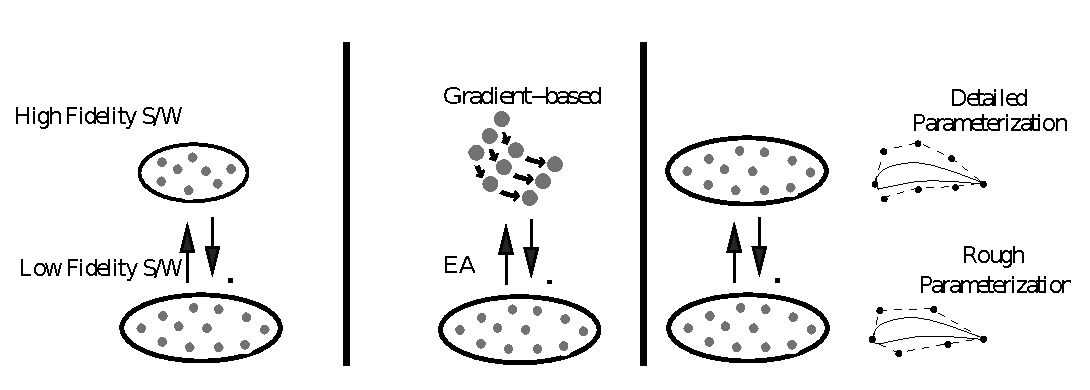
\includegraphics[scale=0.8]{multimodes.eps}
% ------------------------------------------------
    $\mbox{Hierarchical Evaluation~~~~~Hierarchical Search~~~~~~Hierarchical Parameterization}$
%   $\mbox{Hierarchical}~~~~~~~~~~~~~~~~
%    \mbox{Hierarchical}~~~~~~~~~~~~~~~~~~~~
%    \mbox{Hierarchical}$
%   \\
%   $~~~\mbox{ Evaluation }~~~~~~~~~~~~~~~~~~
%    \mbox{   Search   }~~~~~~~~~~~~~~~~~~~
%    \mbox{Parameterization}$
% ------------------------------------------------
    \caption{\HEAs. Schematic representation of the three
            hierarchical schemes.}
    \label{f:allheas}
\end{figure}

Metamodels are automatically incorporated into hierarchical schemes, by just using \MAEAs\ in lieu of \EAs. 
This gives rise to the so--called hierarchical \MAEAs\ (\HMAEAs) in which, in contrast to single level \MAEAs, different \DBs\ of previously evaluated solutions must be kept for the purpose of training the corresponding metamodels on each level.
Each level may optionally apply a \DMAEA\ leading to a Hierarhical \DMAEA\ (\HDMAEA). 
An alternative way is to apply the hierarchy within each deme which gives rise to a Distributed \HMAEA\ (\DHMAEA), fig. \ref{f:dhmaea}.

\begin{figure}[h!]
    \centering
    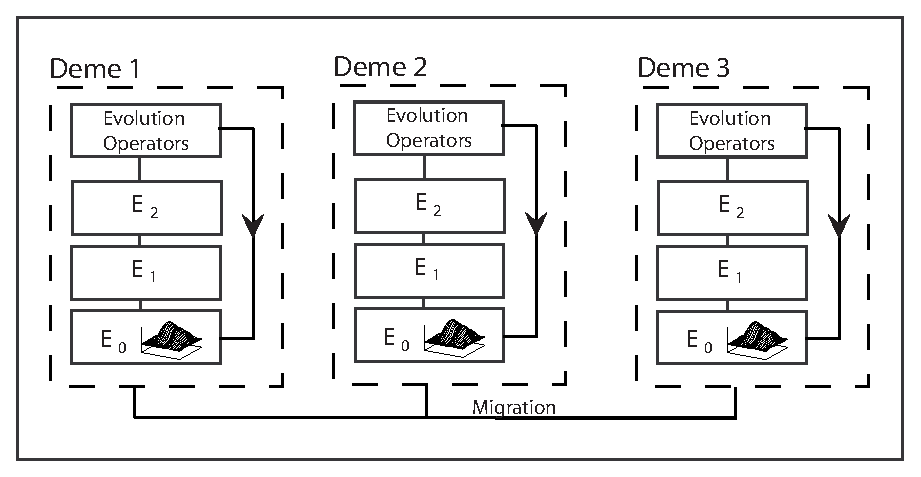
\includegraphics[scale=0.8]{dhmaea.eps}
    \caption{Distributed hierarchical structure with a metamodel ($E_0$),
	     a low--fidelity ($E_1$) and a high--fidelity ($E_2$) 
             evaluation model in each deme.}
    \label{f:dhmaea}
\end{figure}

%
%%=======================================================================
\subsection{Applications of HEAs}
%=======================================================================

Below, two optimization problems solved using the hierarchical evaluation schemes are presented. 
The first one demonstrates the use of the distributed hierarchical evaluation schemes by taking advantage of two different \GPU--enabled code variants that use either single precision arithmetic with a speed--up up to $110\!\times$ (low level) or the mixed precision arithmetic  with a speed--up up to $90\!\times$  (high level). 
In the second case, a hierarhical scheme with a single population is used for the design of an annular compressor cascade.

%
%   Optimization of a 2D isolated airfoil (GPUs)
%
\xeraki The first case deals with the optimal deployment of a four--element airfoil for maximum lift coefficient ($C_L$), as described in \ref{s:maeasapp}, which is herein revisited using the distributed hierarchical evaluation scheme, with and without metamodels.
The low--cost, low--fidelity evaluation tool uses a single precision arithmetic (\GPUS, $E_1$) variant of the \GPU\--enabled Euler software and the high fidelity one uses the mixed precision arithmetic (\GPUM, $E_2$). 
The \CPU\ cost ratio of $E_1$ and $E_2$ is $\sim\!0.48\!:\!1$ for the same computational grid. The low level solver is faster but less accurate due to its single precision arithmetic.
Fig. \ref{f:dhea} compares the convergence history of \DHEA\ and a \DHMAEA\ in terms of \CPU\ cost. For the sake of completeness, the convergence history of the \EA\ of section \ref{s:maeasapp} is also shown in this figure. The three algorithms were configured as follows:
\begin{enumerate}
\item A ($20, 50$) \EA\ using the $E_2$ evaluation model.
\item A \DHEA\ with three ($5, 15$) \EA\ demes. In each generation, the $15$ offspring of each deme were firstly evaluated on $E_1$ and only the top two of them were then re--evaluated on $E_2$.
\item A $3\times (5, 15)$ \DHMAEA. Here in each deme, $15$ offspring were evaluated on the metamodel $E_0$ (i.e. an \RBF\ network), the best $9$ among them were re--evaluated on $E_1$ and only one of them on $E_2$. All local metamodels were trained on individuals previously evaluated on $E_1$.
\end{enumerate}
In both distributed schemes, migration was employed every $8$ generations by exchanging two individuals within any pair of demes. The two emigrants of each deme were selected after ranking the offspring population members in terms of their fitness value, without distinguishing among the evaluation models used to get this value. The migration policy is that, in the destination deme, immigrants replace the worst performing members.

As shown in fig. \ref{f:dhea}, the distributed hierarchical schemes perfoms better than the conventional \EA\ and the combined use of metamodels and hierarchical schemes leads to even better performance.
%
\begin{figure}[ht!]
    \centering
    \includegraphics[scale=1.5]{hmaeas/4elemEaDhea.eps}
    \caption{Optimal deployment of a four--element airfoil for maximum lift 
	     coefficient. Convergence history of the \SOO\ problem, in terms 
	     of \CPU\ cost.}
    \label{f:dhea}
\end{figure}
%


%
%   Optimization of an Annular Cascade
%
\xeraki The second case is concerned with the optimization of a $3D$ annular compressor cascade. 
An existing cascade with $19$ straight blades (chord length equal to $C\!\!=\!\!0.1~m$, stagger angle equal to $51.4^o$) was used as reference. 
The blades were mounted on the casing forming a $t/C\!=\!2\%$ clearance with the stationary hub, \cite{LTT_4_05}. 
The purpose of this study was to redesign the airfoil of the straight blade so as to minimize the mass-averaged pressure loss coefficient $PLC_{ave}$. At each radial position $r$, $PLC$, is defined as
%
\begin{equation}\label{omloss}
    PLC(r) = \frac{ \overline{p}_{t1}(r) - \overline{p}_t(r) }
                  { \overline{p}_{t1}(r) - \overline{p}_{1}(r) }
    \nonumber
\end{equation}
%
where $\overline{p}_{t}(r)$ and $\overline{p}(r)$ stand for the circumferentially mass--averaged total and static pressures.
$PLC_{ave}$ is the average of $PLC(r)$, for all $r\in[r_{hub},r_{shroud}]$.
The cascade airfoil is parameterized using $15$ NURBS control points on each side (pressure and suction sides), $5$ of which were allowed to vary both on the chordwise and the normal to the chord direction, summing up to $20$ design variables.
Geometrical constraints on the airfoil thickness and the mean exit flow angle $\bar{\alpha}_2$ ($\bar{\alpha}_2\!\leq\!53^o$) were imposed.

In this case, a \HMAEA\ with the hierarchical evaluation scheme was used.
The same evaluation tool (in--house Navier--Stokes equations solver, $CFD\!-\!NS$; \CPU\ implementation) was used on both levels, with different spatial resolution and turbulence model. 
In particular, the high--fidelity evaluation model ($E_2$) used the low--Reynolds number Spalart--Allmaras \cite{Spa94} turbulence model on unstructured grids of about $\sim\!1.000.000$ nodes. 
A coarser grid of $\sim\!600.000$ nodes and the same turbulence model with wall functions was used as the low--fidelity evaluation model ($E_1$).
The \CPU\ cost ratio of $E_1$ and $E_2$  $\sim\!0.2:1$.

A $(20,60)$ \HMAEA, with a single population was used.
Fitness inheritance\footnote{Fitness inheritance is a method that approximates the fitness of any offspring from the fitness values of its parents.} and \RBF\ networks supported the \IPE\ process.
During the first generation, all individuals were evaluated on $E_1$
and only the $6$ top of them were re--evaluated on $E_2$. 
In the second generation, the fitness inheritance technique was activated.
The most promising (between $5$ and $10$ of them) members in the
population were re--evaluated on $E_1$ and only the best of them on
$E_2$. Once $100$ previously evaluated individuals on $E_1$ were
archived in the \DB, \RBF\ networks were used in place of fitness
inheritance. 
The \HMAEA\ terminated at $80$ \CPU\ cost units, i.e. $80$ equivalent high level $CFD\!-\!NS$ runs.

Fig. \ref{hmaeas:ntua_blade} illustrates the convergence of the optimization algorithm. The $PLC_{ave}$ values of the reference and optimal blade cascades were found equal to $0.1189$ and $0.0843$, respectively. 
The gain from using the \HMAEA\ is clear since locating the optimal solution at the cost of only $80$ \CPU\ cost units would be otherwise impossible.

\begin{figure}[ht!]
    \centering
    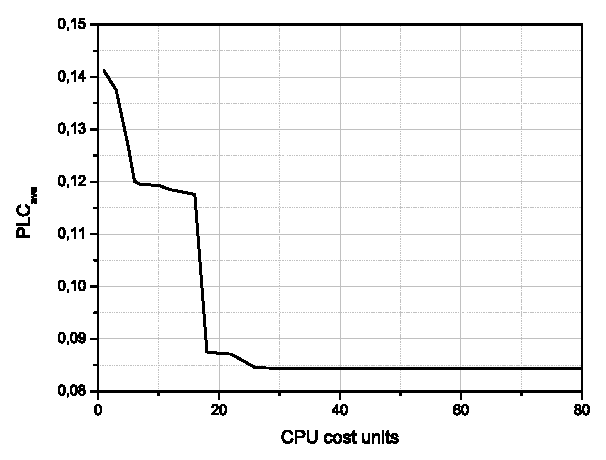
\includegraphics[scale=0.7]{hmaeas/ntua_res.eps}
    \caption{Optimization of an annular cascade. Convergence of the \HMAEA. 
	     One \CPU\ cost unit corresponds to a single computation using the
	     high--fidelity CFD model ($E_2$). From \cite{LTT_4_05}.}
    \label{hmaeas:ntua_blade}
\end{figure}

In fig. \ref{hmaeas:ntua_blade_cpt}, iso--contours of the total pressure loss coefficient $C_{pt}=\frac{\overline{p}_{t1}-\overline{p}_t}{\overline{p}_{t1}-\overline{p}_1}$ are plotted on a transversal cross--section downstream of the blade leading edge, for both the reference and the optimal blades. 
In the redesigned blade, losses induced by the tip clearance vortex are much lower and which lead to the lower $PLC_{ave}$ value, compared to the reference blade.
%
\begin{figure}[h!]
\centering
    \begin{minipage}{.49\linewidth}
       \includegraphics[angle=270,scale=0.3]{hmaeas/r_b_img.eps}
    \end{minipage}
    \begin{minipage}{.49\linewidth}
       \includegraphics[angle=270,scale=0.3]{hmaeas/b_b_img.eps}
    \end{minipage}
    \caption{Optimization of an annular cascade. Total pressure loss
             fields plotted over a transversal cross--section at $0.782\%$
             axial chord downstream of the blade leading edge.
             Computed results for the reference (left) and
             optimal (right) blade. From \cite{LTT_4_05}.}
    \label{hmaeas:ntua_blade_cpt}
\end{figure}
%
The  total pressure field over part of the stator row (four blades) for the optimal blade geometry is shown in fig. \ref{hmaeas:opt_blade_cpt}. 
%
\begin{figure}[h!]
\centering
    \includegraphics[trim=150 50 50 0,clip,angle=270,scale=0.7]{hmaeas/ntuaBv2.eps}
    \caption{Optimization of an annular cascade. Total pressure 
             field on the optimal cascade blade.}
    \label{hmaeas:opt_blade_cpt}
\end{figure}




%#######################################################################
\section[Asynchronous EAs \& MAEAs]
{Asynchronous EAs \& MAEAs}
%#######################################################################
\label{s:AMAEA}

The \EAs\ (\MAEAs, \HMAEAs, etc.) discussed in the previous sections are referred to as synchronous \EAs\ since these are characterized by the notion of ``generation''. The end of each generation acts as a synchronization barrier, regularly during the evolution. 
Upon completion of each generation, the need for synchronization may seriously harm the parallel efficiency of the (synchronous) \EAs. As a remedy to this problem, asynchronous \EAs\ (\AEAs), that overcome the notion of generation and may optimally use all available computational resources, have been proposed.

Below, the \AEA\ originally proposed by the author's group, \cite{LTT_2_040}, which is assisted by metamodels based on the \IPE\ technique (asynchronous \MAEA\, \cite{LTT_2_045}) along with its application to the design of a Hydromatrix\textregistered~ runner are presented.

%=======================================================================
\subsection{AEA: Basic Features}
%=======================================================================
\label{ss:aea}

The \AEA\ presented in \cite{LTT_2_040} utilises a number of search agents located at the nodes of a 2D structured mesh (``supporting mesh'', fig. \ref{f:aeatopo}) with dimensions $n_1\!\times\! n_2$ which is considered to be periodic along its two pairs of opposite sites ($n_1$, $n_2$ are user--defined even integers). 
\begin{figure}[h!]
\centering
    \includegraphics[angle=0,scale=0.6]{topo.eps}
    \caption{Asynchronous EA. A $6\!\times\!4$ supporting mesh. Poles 
	     correspond to circles filled in black.}
    \label{f:aeatopo}
\end{figure}

The mesh is divided into a number ($n_1 n_2 / 4$) of overlapping demes ($\Dp$) with six nodes each. Each deme comprises five search agents and a single pole, leading to $N_{poles}\!=n_1n_2/4$ and $N_{agents}\!=\!3n_1n_2/4$.
The demes overlapping enables the inter--deme communication and exchange of information among them.
Each pole acts as the front--end of its deme, where the best--so--far individual (local best) computed by the search agents of this deme is stored and, through the local best, affects the formation of new candidate solutions. 
On the other hand, search agents undertake evaluations, generate new candidate solutions (based on evolution operators applied within each deme) and are responsible for updating the information stored in the poles (according to the outcome/result of each evaluation).

The \AEA\ algorithm, which is suitable for either \textit{Cluster} or \textit{Grid Computing} with $N_{CPU}$ available processors, is presented below:

%
%.........................................................
\begin{namedalgorithm}{AEA}
{Asynchronous Evolutionary Algorithm}{}
%.........................................................
\item[Start Algorithm]\label{aea:start}
$N_{CPU}$ randomly generated individuals are associated with
$N_{CPU}$ agents and undergo evaluation on all available processors.
%
\item[Receive]\label{aea:receive}
The evaluation of an individual $(\vect{x}_a,\vect{F}(\vect{x}_a))$ (the subscript $a$ stands for agent) is completed and the corresponding \CPU\ ($\CPU_{\vect{x}_a}$) becomes instantaneously idle.
%
\item[Elitism]
The elite archival set, $\set{P}_a$, is updated accordingly.
%
\item[Pole Displacement]
Through an intra--deme process, a decision on whether the just evaluated individual $\vect{x}_a$ must displace $\vect{x}_p$ which is stored at the corresponding pole(s) is made. 
To this end, $\vect{F}(\vect{x}_a)$ is compared with $\vect{F}(\vect{x}_p)$, based on dominance criteria (\MOO\ problems).
%
\item[Update Ages]
Agents' and poles' ages are updated. The age $A_k$ of each agent $k$
with $k\!\in\![1,N_{agents}]$ is defined as the difference between
the serial number of the last evaluation carried out for this agent
and the serial number of the current evaluation. Each pole takes on
the average age of its agents, 
\begin{equation}\label{aea_poleage}
    A_p = \frac{1}{5} \sum_{k \in \Dp} A_k,~\mbox{with}~p\in[1,N_{poles}]
    \nonumber
\end{equation}
%
\item[Update Priorities]
The priority of each pole $Pr_p$ (which is equal to the priority of its deme) is the product of the age-- and a cost--based priorites, as
\begin{equation}
    Pr_p=Pr_p^{age}Pr_p^{cost}
    \nonumber
\end{equation}
with
\begin{equation}
    Pr_p^{age} = \frac{A_p}{\mbox{max}~(A_1,\cdots,A_{N_{poles}})}
    \mbox{ and }   
    Pr_p^{cost}= \frac{\phi_p}{\phi_{max}-\phi_{min}}
    \nonumber
\end{equation}
%
where $\mbox{max}~(A_1,\cdots,A_{N_{poles}})$ denotes the maximum age of all poles, $\phi_p=\phi(\vect{x}_p)$ is the scalar cost function associated with pole $p$, and
$\phi_{max}=\mbox{max}~(\phi_1,\cdots,\phi_{N_{poles}})$,
$\phi_{min}=\mbox{min}~(\phi_1,\cdots,\phi_{N_{poles}})$ are the
maximum and minimum $\phi$ values among all poles, respectively.
%
\item[Select New Deme \& Agent]\label{aea:selection}
The agent with the maximum age, within the deme with the maximum priority, is selected as the one where the new individual to undergo evaluation must be formed.
%
\item[Recombination \& Mutation]\label{aea:xover}
The new individual is formed by superimposing the weighted
difference between two agents of the deme selected in \ref{aea:selection} to the individual associated with the pole $\vect{x}_p$, as
%
\begin{equation}\label{aea_xover}
    \vect{x}_a^{new, temp} = \vect{x}_p +
    \omega_r (\vect{x}_{k_1} - \vect{x}_{k_2}), ~\mbox{with}~
    k_1,k_2 \in \Dp^n ~\&~ k_1\neq k_2
\end{equation}
%
where $\omega_r\!\in\![0,1]$. A non--uniform mutation scheme, with a
user--defined probability is, then, applied to $\vect{x}_a^{new, temp}$, 
yielding $\vect{x}_a^{new}$.
%
\item[Assign Evaluation]
Assign the evaluation of $\vect{x}_a^{new}$ on the idle \CPU,
$\CPU_{\vect{x}_a}$.
%
\item[Termination] If the maximum number of evaluations is reached
or the elite set does not further improve for a user--defined
number of successive evaluations the algorithm terminates.
Otherwise, it continues from step \ref{aea:receive}.
%...................
\end{namedalgorithm}
%...................

%
%-----------------------------------------------------------------------
\subsection[Implementation of Metamodels in AEA]
{Implementation of Metamodels in AEA}
%-----------------------------------------------------------------------
\label{ss:amaea}

The efficiency of the \AEA\ can be significantly improved by employing metamodels, according to the \IPE\ technique.
In the synchronous variants of \EAs\ which have been discussed in previous sections, the \IPE\ technique is applied for inexactly pre--evaluating all the population at each generation and screen out the non--promising individuals. 
The lack of generations in \AEA\ requires a ``different'' way of performing the \IPE\ of candidate solutions.

Thus, the asynchronous metamodel--assisted \EA\ (\AMAEA, \cite{LTT_2_045}), 
starts as an \AEA\ until a user--defined number of exact evaluations are 
completed and archived in \DB. Then, the \IPE\ phase begins. 
During \IPE, instead of generating a single new individual in the agent 
selected to undergo evaluation (step \ref{aea:xover}), $N_{IPE}$ trial 
individuals are generated and inexactly pre--evaluated on the metamodel. 
The ``best'' of them, according to the metamodel is selected to undergo evaluation. 
This algorithm, which replaces step \ref{aea:xover}, is presented below:
%
%.................................................
\begin{namedalgorithm}{AMAEA}{Asynchronous \MAEA}{}
%.................................................
\item[Generate and approximately evaluate $N_{IPE}$ trial individuals]
For each trial individual $t$, $t\!\in\![1,N_{IPE}]$, the following
actions are taken:
%
\begin{algorithm}
\item[Recombination \& Mutation]
Each trial individual ($\vect{x}_a^t$) is generated according to the
recombination and mutation schemes of step \ref{aea:xover} and eq.
\ref{aea_xover}.
%
\item[Inexact Evaluation]
For $\vect{x}_a^t$, a local metamodel is trained on a small, user--defined, number of data selected from the \DB. The training pattern's selection is based on the algorithm described in subsection \ref{tps}. Then, approximate objective values, $\apprx{\vect{F}}(\vect{x}_a^t)$, are computed.
\end{algorithm}
%
\item[Select Trial Individual] 
The ``best'' trial individual according to the metamodel, ($\vect{x}_a^t$, $\apprx{\vect{F}}(\vect{x}_a^t)$), $t\!\in\![1,N_{IPE}]$ is selected to undergo evaluation on the problem--specific model. 
In \MOO\ problems, this selection is based on dominance and strength criteria.
%...................
\end{namedalgorithm}
%...................

%
%-----------------------------------------------------------------------
\subsection{Applications of AEAs}
%-----------------------------------------------------------------------

This section presents two optimization problems solved using \AEAs\ and \AMAEAs. 
The first case demonstrates the gain from the use of metamodels on \AEA\ on the design of an isolated airfoil whereas, in the second case, the \AMAEA\ is used for the design--optimization of a Hydromatrix\textregistered~runner blade.

%
%   Optimization of an isolated airfoil
%
\xeraki The first case is dealing with the two--objective shape optimization of an isolated airfoil for minimum $C_D$ and maximum $C_L$.
The flow conditions are $M_{\infty}\!=\!0.3$, $\alpha_{\infty}\!=\!4^o$ and $Re_c \!=\! 5 \cdot 10^6$. The $CFD\!-\!NS$ solver was used. The airfoil is parameterized using $24$ design variables. Geometrical constraints were imposed
on the airfoil thickness.

This case was studied using \AEA\ and \AMAEA, both of them on a $12\!\times\!10$ supporting mesh. \AMAEA\ employed the \IPE\ technique by generating $N_{\IPE}\!=\!15$ trial members for each individual to be evaluated. 
The comparison of the evolution of the hypervolume indicator $I_H$ for the \AEA\ and the \AMAEA\ along with the front of the non--dominated solutions obtained using the \AMAEA\ are shown fig. \ref{aeas:isol2d}. 
From this figure, it is clear that \AMAEA\ outperforms \AEA.

\begin{figure}[!ht]
\centering
\begin{minipage}{1.0\linewidth}
    \centering
    \begin{minipage}{0.48\linewidth}
        \includegraphics[scale=1.2]{amaea/amaeaVsAea.eps}
    \end{minipage}
    \begin{minipage}{0.48\linewidth}
        \includegraphics[scale=1.2]{amaea/paretoGeamaea.eps}
    \end{minipage}
\end{minipage}
\begin{minipage}{1.0\linewidth}
    \centering
    \begin{minipage}{0.32\linewidth}
        \includegraphics[trim=0 0 0 90,clip,scale=0.7]{amaea/airfoil01.eps}
        $C_L\!=\!0.508, C_D\!=\!0.0107$
    \end{minipage}
    \begin{minipage}{0.32\linewidth}
        \includegraphics[trim=0 0 0 90,clip,scale=0.7]{amaea/airfoil02.eps}
        $C_L\!=\!0.9047, C_D\!=\!0.0142$
    \end{minipage}
    \begin{minipage}{0.32\linewidth}
        \includegraphics[trim=0 0 0 90,clip,scale=0.7]{amaea/airfoil03.eps}
        $C_L\!=\!1.0739, C_D\!=\!0.018$
    \end{minipage}
\end{minipage}
    \caption{Shape optimization of a 2D isolated airfoil. Comparison of
             the convergence of the hypervolume indicator for the \AEA\
             and the \AMAEA\ and the computed front of non--dominated
             solutions. Three airfoil shapes corresponding to
             three points of the computed front of non--dominated
             solutions are also shown. From \cite{LTT_2_045}.}
    \label{aeas:isol2d}
\end{figure}
%

%
% Design of a Hydromatrix runner 
%
\xeraki The second case presents the design--optimization of a Hydromatrix\textregistered~runner blade using \AMAEA. 
Compared to the case presented in section \ref{s:maeasapp}, the new design is carried out at different operating points and is handled as a three objective problem (min $F_1$, $F_2$ and $F_3$).
The three objective functions are the weighted sum of metrics $f_1$, $f_2$ and $f_3$ (for the three operating points), as
\begin{equation}
   F_j = \sum_{i=1}^3 w^{OP_i} f_j^{OP_i}, ~~~ j=1,2,3
   \nonumber
\end{equation}
with $w^{OP_1}=1.0,~ w^{OP_2}=w^{OP_3}=0$ for $F_1$ 
and  $w^{OP_1}=1.0,~ w^{OP_2}=w^{OP_3}=0.1$ for both $F_2$ and $F_3$.
The $f_1$, $f_2$, $f_3$ metrics have been defined in section \ref{s:maeasapp}.

The design was performed using an \AMAEA\ with a $10\!\times\!10$ supporting mesh, i.e. with $75$ agents and $25$ poles on $16$ interconnected \CPUs\ and a stopping criterion of $2000$ CFD--based evaluations.
The \IPE\ technique was applied after the first $300$ non--failed evaluations were stored in the \DB, by generating and approximately evaluating $N_{IPE}\!=\!8$ trial members. 

Fig. \ref{f:amaeaFront} presents the front of non--dominated solutions computed by the \AMAEA\ at the cost of $2000$ CFD evaluations. The runner's blades along with the pressure field at the best efficiency point ($OP_1$) for an indicative solution from this front (point marked with the cube) are shown in fig. \ref{f:amaeaBlade}.
Fig. \ref{f:amaeaStats} presents statistical results on the evaluations performed by each agent (left part) and deme (right part), expressed as percentage (\%) of the total number of evaluations. From this figure, one may notice that the evaluations are almost equally shared among the $25$ demes. Also, as expected, unlike agents shared by two demes (see fig. \ref{f:aeatopo}), those belonging exclusively to a single deme usually perform less evaluations.

In this case, the important thing is that the available \CPUs\ were used without idle periods of time, since no synchronization occurs in \AMAEA; so, this optimization problem practically had $100\%$ parallel efficiency.

\begin{figure}
    \centering
    \includegraphics[trim=100 40 40 40,scale=0.5, angle=-90]{amaea/paretoA.eps}
    \caption{Three--objective optimization of a Hydromatrix\textregistered~
             runner. Front of the computed non--dominated solutions, 
	     at the end of 2000 CFD--based evaluations. From \cite{LTT_3_104}.}
    \label{f:amaeaFront}
\end{figure}

\begin{figure}
    \centering
    \includegraphics[trim=100 0 0 0,angle=-90,scale=0.5]{amaea/matrixRes.eps}
    \caption{Three--objective optimization of a Hydromatrix\textregistered~
             runner. View of the blades of the runner for the selected 
	     solution (point marked with a cube in fig. \ref{f:amaeaFront}) 
	     along with the pressure field at $OP_1$. From \cite{LTT_3_104}.}
    \label{f:amaeaBlade}
\end{figure}
%
\begin{figure}[h!]
\centering
    \begin{minipage}{.49\linewidth}
       \includegraphics[angle=-90,scale=0.4]{amaea/agent_evals.eps}
    \end{minipage}
    \begin{minipage}{.49\linewidth}
       \includegraphics[angle=-90,scale=0.4]{amaea/demes_evals.eps}
    \end{minipage}
    \caption{Three--objective optimization of a Hydromatrix\textregistered~ 
	     runner. Statistical results on the evaluations performed by each
             agent (left) and deme (right) of the supporting mesh, as a 
             percentage of the total number of evaluations. 
             From \cite{LTT_3_104}.}
    \label{f:amaeaStats}
\end{figure}
%


%#######################################################################
\section*{Acknowledgement}
%#######################################################################

The optimization of the Hydromatrix\textregistered~design cases was supported by Andritz HYDRO (Linz, Austria and Vevey, Switzerland), in the framework of direct collaborations between NTUA and the aforementioned company and/or the EU funded project ``HYDROACTION''.

%
%   B I B L I O G R A P H Y
%
\bibliography{vki2012,ltt}
\bibliographystyle{plain}



%%%%%%%%%%%%%%%%%%%%%%%%%%%%%%%%%%%%%%%%%%%%%%%%%%%%%%%%%%%%%%%%%%%%%%%%
\end{document}
%%%%%%%%%%%%%%%%%%%%%%%%%%%%%%%%%%%%%%%%%%%%%%%%%%%%%%%%%%%%%%%%%%%%%%%%
